


\pbn
\section{Trade can make everyone better off}\label{sec:mankiw}	
\begin{minipage}{0.5\linewidth}	
	\begin{center}
		\includegraphics[width=.8\linewidth]{../../../pic/nmankiw}\captionof{figure}{N. Gregory Mankiw}\label{fig:mankiw1}\note{Source: \url{http://scholar.harvard.edu/mankiw/}}
	\end{center}
\end{minipage}
\begin{minipage}{0.5\linewidth}	
	\begin{center}
		\includegraphics[width=.5\linewidth]{../../../pic/mankiw-principles}\captionof{figure}{N. Gregory Mankiw}\label{fig:mankiw2}\note{Source: \cite{Mankiw2020Principles}}
	\end{center}
\end{minipage}

\textbf{N. Gregory Mankiw }(*1958) is one of the most influential economists. In his best-selling textbook \textit{Principles of Economics} \citep[see][]{Mankiw2020Principles} he claims ten principles of economics of which one is entitled \textit{Trade can make everyone better off} which he explains as follows:

\pbn
\zitat{``You have probably heard on the news that the Japanese are our competitors in the
	world economy. In some ways, this is true, for American and Japanese firms do
	produce many of the same goods. Ford and Toyota compete for the same customers in the market for automobiles. Compaq and Toshiba compete for the same customers in the market for personal computers. 
	
	Yet it is easy to be misled when thinking about competition among countries.
	Trade between the United States and Japan is not like a sports contest, where one
	side wins and the other side loses. In fact, the opposite is true: Trade between two
	countries can make each country better off.
	
	To see why, consider how trade affects your family. When a member of your
	family looks for a job, he or she competes against members of other families who
	are looking for jobs. Families also compete against one another when they go
	shopping, because each family wants to buy the best goods at the lowest prices. So,
	in a sense, each family in the economy is competing with all other families.
	
	Despite this competition, your family would not be better off isolating itself
	from all other families. If it did, your family would need to grow its own food,
	make its own clothes, and build its own home. Clearly, your family gains much
	from its ability to trade with others. Trade allows each person to specialize in the
	activities he or she does best, whether it is farming, sewing, or home building. By
	trading with others, people can buy a greater variety of goods and services at
	lower cost.
	
	Countries as well as families benefit from the ability to trade with one another.
	Trade allows countries to specialize in what they do best and to enjoy a greater variety of goods and services. The Japanese, as well as the French and the Egyptians
	and the Brazilians, are as much our partners in the world economy as they are our
	competitors'' \citep[p. 8-9]{Mankiw2020Principles}}


\pbn
\section{Reasons for trade}{\label{sec:reasons}\label{Reasons for trade}
	
	Before we come to reasons for trade in further detail, let us name five important explanations or reasons why trade takes place between countries. Of course, the list is incomplete.
	
	\paragraph{Differences in technology}
	Advantageous trade can occur between countries if they differ in their technological abilities to produce goods and services. Technology refers to the techniques used to turn resources (labor, capital, land) into outputs. The basis for trade in the Ricardian Model of Comparative Advantage is differences in technology. We will come back to this in \autoref{sec:ricardo} in more detail.
	
	\paragraph{Differences in endowments}	
	Trade between countries also occur because countries differ with respect to their endowments of resources which refers to the skills and abilities of a country's workforce, the natural resources available within its borders, and the sophistication of its capital stock such as machinery, infrastructure, and communications systems. The basis for trade in the pure exchange models (see \autoref{sec:exchange-economy}) and the Heckscher-Ohlin Model (see \autoref{sec:ho}) is differences in resource endowments.
	
	\paragraph{Differences in demand}
	Trade between countries occurs because the demands or preferences differ between countries. Individuals in different countries may have different preferences or demands for various products. The Asian people are likely to demand more rice than Americans, even if facing the same price. Czech and German people may demand more beer, the Dutch more wooden shoes, and the Japanese more fish than Americans, even if they all faced the same prices.
	
	\paragraph{Economies of scale in production}
	The existence of economies of scale in production is sufficient to generate advantageous trade between two countries. Economies of scale refer to a production process in which production costs fall as the scale of production rises. This feature of production is also known as \textit{increasing returns to scale}. Economics of scale play a huge role in Paul Krugman's \textit{New Trade Theory} which we discuss later.  
	
	\paragraph{Existence of Government Policies}
	Government tax and subsidy programs can be sufficient to generate advantages in production of certain products. In these circumstances, advantageous trade may arise solely due to differences in government policies across countries. We will touch the impact of tariffs and regulations in \autoref{sec:policy}.
	
	\pbn
	\section{Microeconomic preliminaries}\label{sec:Microeconomic_foundation}
	
	\subsection{Production possibility frontier curve}
	
	\begin{minipage}{0.6\linewidth}	
		The production possibility frontier curve (PPF) is a graphical representation showing all the possible options of output for two products that can be produced using all the given resources and factors of production are fully and efficiently utilized per unit time. The PPF is the boundary between the combinations of goods and services that can be produced and the combinations that cannot.
		The PPF is a valuable tool for illustrating the effects of scarcity and its consequences, as it can teach us a lot about production efficiency, opportunity costs, and tradeoffs between different choices. The PPF is (usually) concave because not all resources are equally productive in all activities.
	\end{minipage}
	\begin{minipage}{0.4\linewidth}	
		\begin{figure}[H]
			\begin{center}
				\begin{tikzpicture}
					\begin{axis}[
						scale = 0.6,
						xmin = 0, xmax = 9,
						ymin = 0, ymax = 9,
						axis lines* = left,
						xtick = {0}, ytick = \empty,
						axis on top,
						clip = false,
						]
						% Production-possibility frontier
						\addplot [domain = 0:9, restrict y to domain = 0:9, samples=10000, color = blue, very thick, name path = frontier]{(49-x^2)^0.5};
						\addplot [domain = 0:9, restrict y to domain = 0:9, draw = none, name path = axis]{0};
						
						% Colouring areas
						\addplot [yellow,  opacity = 0.1] fill between [of = frontier and axis];
						
						% Labels
						\node [right] at (current axis.right of origin) {$A$};
						\node [above] at (current axis.above origin) {$B$};
						\tkzDefPoint(1,1){A}
						%			\tkzLabelPoint[right,font=\tiny](A){(100,100)}
					\end{axis}
				\end{tikzpicture}
			\end{center}	
			%	\caption{The production possibilities curve}
		\end{figure}
	\end{minipage}
	
	
	\pbn
	\exextoc{Understanding production}{		
		\begin{minipage}{0.6\linewidth}	
			\abcx{
				\item The figure shows a PPF and five conceivable production points, $C_i$, where $i\in \{1,\dots,5\}$. 
				Explain the figure using the following terms:  \textit{attainable point; available resources, unattainable, inefficient, efficient point}.
				\item What would happen to the PPF if the technology available in a country and needed for the production process became better?
				\item What would happen to the PPF if the resources available in a country and needed in the production process of both goods shrank?
				\item What would happen to the PPF if the resources (technology) available in a country that are needed in the production process$\dots$ 
				\itex{
					\item $\dots$ for both goods increased (improved)?
					\item $\dots$ for good A shrank (got worse)?
					\item $\dots$ for good B increased (improved)?
				}
				\item Does the shape of the PPF tell us anything about economies of scale in the production process?
				\item The figure on the right shows an extreme PPF. How can such a PPF be explained?
			}
		\end{minipage}
		\begin{minipage}{0.4\linewidth}	
			\begin{center}
				\begin{tikzpicture}
					\begin{axis}[
						scale = 0.8,
						xmin = 0, xmax = 9,
						ymin = 0, ymax = 9,
						axis lines* = left,
						xtick = {0}, ytick = \empty,
						axis on top,
						clip = false,
						]
						% Production-possibility frontier
						\addplot [domain = 0:9, restrict y to domain = 0:9, samples=10000, color = blue, very thick, name path = frontier]{(49-x^2)^0.5};
						\addplot [domain = 0:9, restrict y to domain = 0:9, draw = none, name path = axis]{0};
						
						% Colouring areas
						\addplot [yellow,  opacity = 0.1] fill between [of = frontier and axis];
						
						%			\addplot [domain = 0:9, restrict y to domain = 0:9, samples=10000, color = red, very thick, name path = frontier]{(49-x^2)^2}
						
						\draw [fill] (7,0) circle [radius=.1];
						\node [left] at (7,0) {$C_1$};
						
						\draw [fill] (2.5,4.5) circle [radius=.1];
						\node [right] at (2.5,4.5) {$C_2$};
						
						%			\draw [fill] (4.5,4.5) circle [radius=.1];
						%			\node [right] at (4.5,4.5) {$C_3$};
						
						\draw [fill] (4.5,5.35) circle [radius=.1];
						\node [right] at (4.5,5.35) {$C_4$};
						
						\draw [fill] (0,7) circle [radius=.1];
						\node [below] at (0,7) {$C_3$};
						
						\draw [fill] (7,7) circle [radius=.1];
						\node [below] at (7,7) {$C_5$};
						
						% Labels
						\node [right] at (current axis.right of origin) {$A$};
						\node [above] at (current axis.above origin) {$B$};
						\tkzDefPoint(1,1){A}
						%			\tkzLabelPoint[right,font=\tiny](A){(100,100)}
					\end{axis}
				\end{tikzpicture}
				\vfill
				
				\begin{tikzpicture}[scale=.5]
					
					\draw [<-] (0,6) node [left] {$B$} -- (0,0);
					\draw [->] (0,0) -- (6,0) node [below] {$A$};
					%	\node [left] at (0,6.45) {$P$};
					%	\node [below] at (5.05,0) {$P'$};
					%	\node [left] at (4.3,3.2) {$x^n$};
					%	\node [below] at (2.4,5.4) {$y^f$};
					%	\node [right] at (5.75,3.4) {$x^f$};
					\draw [color = blue, very thick] (5,0) -- (5,5);
					\draw [color = blue, very thick] (0,5) -- (5,5);
					%	\draw (4.45,5.3) to [out=-90, in=140] (5.75,3.2) to [out=-40, in=160] (7.7,2.2);
					%	\draw (4.15,4.3) to [out=-90, in=120] (4.55,3) to [out=-60, in=160] (7.4,1.1);
					%	\draw (0,6.45) to [out=0, in=115] (4.4,3.2) to [out=-65, in=90] (5.05,0);
				\end{tikzpicture}
			\end{center}	
		\end{minipage}
	}
	
	
	
	\solx{Understanding production}{
		\abcx{
			\item Any point that lies either on the production possibilities curve or to the left of it is said to be an attainable point: it can be produced with currently available resources. Production points that lie in the yellow shaded area are said to be unattainable because they cannot be produced using currently available resources. These points represent an inefficient production, because existing resources would allow for production of more of at least one good without sacrificing the production of any other good. An efficient point is one that lies \textbf{on} the production possibilities curve. At any such point, more of one good can be produced only by producing less of the other. 
			\item Task solved in class.
			\item Task solved in class.
			\item Task solved in class.
			\item With economies of scale, the PPF would curve inward, with the opportunity cost of one good falling as more of it is produced. A straight-line (linear) PPF reflects a situation where resources are not specialized and can be substituted for each other with no added cost. With constant returns to scale, there are two opportunities for a linear PPF: if there was only one factor of production to consider or if the factor intensity ratios in the two sectors were constant at all points on the production-possibilities curve. 
			\item Here is one example: Suppose a country that is endowed with two factors of production and that one factor can only be used for producing good A and the other factor can only be used to produce good B. 
		}
	}
	
	
	\pbn
	\subsection{Indifference curves}
	
	
	\begin{minipage}{0.6\linewidth}	
		Combinations of two goods that produce the same utility are plotted on an indifference curve. All points along an indifference curve produce the same utility for a country's consumers.
		Consumers are indifferent between points on the indifference curve. These curves are derived from utility functions that explain consumers' desire to consume different bundles of the two goods.
	\end{minipage}
	\begin{minipage}{0.4\linewidth}	
		\begin{center}
			\begin{tikzpicture}[scale=0.7]
				% Axis
				\draw [->] (0,0) node [below] {0} -- (0,0) -- (7.5,0) node [below] {A};
				\draw [->] (0,0) node [below] {0} -- (0,0) -- (0,5.5) node [above] {B};
				% Indifference curve
				\draw (0.3,5) to [out=280,in=175] (5.5,0.5);
				\node [right] at (5.5,0.5) {$IC$};
			\end{tikzpicture}
		\end{center}
	\end{minipage}
	
	
	\itex{
		\item The slope of an indifference curve indicates the rate at which two goods can be substituted without changing the consumers' utility. In technical terms, the marginal rate of substitution is equal to the absolute value of the slope of an indifference curve. It is the maximum quantity of a good that a consumer is willing to give up in order to obtain one additional unit of another good. 
		\item We assume that each consumer seeks the highest possible indifference curve, because the higher, or farther to the right, an indifference curve lies in a coordination system, the higher the utility level it represents.
	}
	
	\exextoc{Understanding indifference curves}{
		\begin{minipage}{0.7\linewidth}	
			\abcx{
				\item Which indifference curve in the figure on the right represents the highest utility level? Explain your decision.
				\item Suppose two goods are perfect substitutes\footnote{Two goods are substitutes if they can be used for the same purpose or provide the same utility to the consumer}. Draw the indifference curves for perfect substitutes. 
				\item Suppose two goods are perfect complements\footnote{Two goods are complements if they go well together and the demand for one good is related to the demand for another good. A perfect complement is a good that must be consumed together with another good}. Draw the indifference curves for perfect complements. 
				\item Suppose you have a fixed income $I=10$ that you can spend on consuming two goods $x, y$ at certain prices $p_x=1, p_y=1$. Draw the budget line consisting of all possible combinations of two goods that a consumer can buy at certain market prices by allocating his income. Using indifference curves, sketch what each consumer should consume to maximize utility.
			}
		\end{minipage}
		\begin{minipage}{0.25\linewidth}	
			\begin{center}
				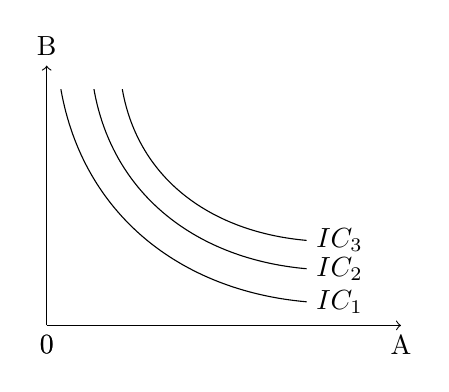
\begin{tikzpicture}[scale=0.6]
					% Axis
					\draw [->] (0,0) node [below] {0} -- (0,0) -- (7.5,0) node [below] {A};
					\draw [->] (0,0) node [below] {0} -- (0,0) -- (0,5.5) node [above] {B};
					% Indifference curve
					\draw (0.3,5) to [out=280,in=175] (5.5,0.5);
					\node [right] at (5.5,0.5) {$IC_1$};
					\draw (1,5) to [out=280,in=175] (5.5,1.2);
					\node [right] at (5.5,1.2) {$IC_2$};
					\draw (1.6,5) to [out=280,in=175] (5.5,1.8);
					\node [right] at (5.5,1.8) {$IC_3$};
				\end{tikzpicture}
			\end{center}
			\vfill
		\end{minipage}
	}
	
	\pbn
	\solx{Understanding indifference curves}{
		\begin{minipage}{0.4\linewidth}
			\abcx{
				\item $IC_3$ represents the highest level of utility. $IC_1$ represents the lowest level of utility.  
				\item  Task solved in class.
				\item  Task solved in class.
				\item The budget line can be sketched into a y-x plot by solving $p_xx+p_yy=I$ for y: $$y=\frac{I}{p_y}-\frac{p_x}{p_y}x$$
			}
		\end{minipage}
		\begin{minipage}{0.6\linewidth}
			\begin{center}
				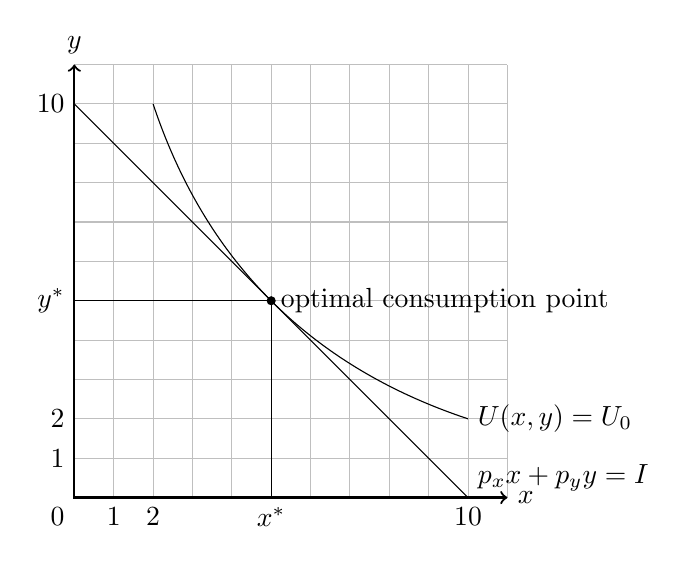
\begin{tikzpicture}[scale=0.5]
					\draw [color=gray!50]  [step=10mm] (0,0) grid (11,11);
					\draw[thick,<->] (0,11) node[above]{$y$}--(0,0)--(11,0) node[right]{$x$};
					\node [below left] at (0,0) {$0$};
					\node [below] at (5,0) {$x^{*}$};
					\node [below] at (1,0) {1};
					\node [below] at (2,0) {2};
					\node [below] at (10,0) {10};
					\node [right] at (5,5) {optimal consumption point};
					\draw [fill] (5,5) circle [radius=.1];
					\node [left] at (0,1) {1};
					\node [left] at (0,2) {2};
					\node [left] at (0,10) {10};
					\node [left] at (0,5) {$y^{*}$};
					\draw(0,10)--(10,0);
					\node [right] at (10,.5) {$p_xx+p_yy=I$};
					\draw(0,5)--(5,5)--(5,0);
					\draw(2,10) ..controls (3.33,6) and (6,3.33) .. (10,2) node[right]{$U(x,y)=U_0$};
				\end{tikzpicture}
			\end{center}
		\end{minipage}
	}
	
	\pbn
	\subsection{Utility maximization}
	
	\exextoc{Utility maximization}{
		\begin{minipage}{0.3\linewidth}
			\begin{center}
				\includegraphics[width=0.9\linewidth]{../../../pic/utility-max}
			\end{center}
		\end{minipage}
		\begin{minipage}{0.7\linewidth}
			The figure on the right is from \citet[ch. 4] {Emerson2020Intermediate}. Match the following sentences to the respective points in the figure.
			\abcx{
				\item Optimal bundle.
				\item Can do better by trading some B for some A.
				\item Can do better by trading some B for some A.
				\item Unaffordable.
			}
		\end{minipage}
	}
	
	\solx{Utility maximization}{
		See \citet[p. 46]{Emerson2020Intermediate}.
	}
	
	Utility maximization is a matter of selecting a combination of two goods that satisfies two conditions:
	\enux{\item The point at which utility is maximized must be within the attainable region defined by PPF or affordable when there is a budget to spend.
		\item The point at which utility is maximized must be on the highest indifference curve consistent with
		condition.}
	
	
	
	\pbn
	\subsection{Important insights}
	
	
	
	I emphasize important insights, principles, and the alike in \textit{Eurekas}\footnote{The word \textit{Eureka} is a famous exclamation attributed to the philosopher Archimedes of Syracuse (287-212 B.C.) that denotes a sudden or unexpected realization of a problem solution}:
	
	\heux{Price in autarky}{
		The price relation in autarky is equal to the slope of the PPF at the point where it is tangent to the indifference curve.
	}
	\heux{Utility maximizing production}{
		The production point that maximizes utility is the point where the PPF is tangent to the price relation. This is true in autarky and under free trade.
	}
	\heux{Consumption under free trade}{
		Starting from the production point, a country will trade goods until the world price relation is tangent to the indifference curve.
	}
	
	\exextoc{Sketch important insights}{
		Review the three key findings by sketching an explanatory graphic for each finding.
	}
	
	%\newpage
	%\minipx{.6}{\includegraphics[width=0.9\linewidth]{$HOME/Dropbox/hsf/pic/micro/max_ic}}{.3}{Utility maximization is thus a matter of selecting a combination of two goods that satisfies two conditions:
	%	\enux{\item The point at which utility is maximized must be within the attainable region defined by the CPF the PPF.
	%		\item The point at which utility is maximized must be on the highest indifference curve consistent with
	%		condition.}}
	
	
	
	
	
	
	%\section{Trade Models}
	\pbn
	\section{Exchange economy}\label{sec:exchange-economy}
	
	
	\subsection{A simple barter model}
	
	The simplest example to show that trade can be beneficial to people is the barter model. In trade, barter is a system of exchange in which participants in a transaction directly exchange goods or services for other goods or services without using a medium of exchange, such as money. 
	
	
	\begin{minipage}{0.4\linewidth}	\begin{center}
			\includegraphics[width=.9\linewidth]{../../../pic/ie/weiswurst}\note{Source: \href{https://upload.wikimedia.org/wikipedia/commons/0/08/Weisswurst_Brezn_Senf.jpg}{Wikipedia}}
		\end{center}
	\end{minipage}
	\begin{minipage}{0.6\linewidth}	\textbf{Stylized example of weißwürst and pretzels}\\
		Suppose there are two people, Anton (A) and Barbara (B). Anton has 10 Weißwürste (white sausages) and Barbara has 10 pretzels. Together, they are isolated from the rest of the world for a few days due to a natural disaster. Fortunately, they both have additional access to an endless supply of sweet mustard and beer and they now wonder how to share pretzels and sausages the upcoming days. Let's assume that both of them accept only a white sausage eaten together with a pretzel. That is, eating two pretzels with a sausage is no better than eating a pretzel and a sausage. After some discussion, Barbara gives 5 pretzels and Anton gives Barbara 5 sausages in return. They strongly believe that there is no better way to share food.
	\end{minipage}
	
	
	This example shows that trade can be beneficial for two individuals. Here we basically assume two things. Firstly, two individuals can trade and secondly, they are endowed with different goods. 
	
	\pbn
	\exextoc{How Barbara and Anton trade}{
		\abcx{
			\item Visualize the starting point of Anton and Barbara as described above in a two-way plot where the Anton's initial endowment with sausages is drawn on the y-axis and Barbara's endowment with pretzels is drawn on the x-axis. 
			\item Given their preferences, mark the consumption point after goods were traded. Also, draw in the plot how much Anton and Barbara \textit{exports} and \textit{imports}, respectively. 
			\item Sketch the indifference curve of both individuals in the consumption point after trade has happened.
			\item Draw a new two-way plot and assume that Barbara now gives away 2 pretzels in order to receive one sausage. Mark the resulting consumption points of Anton and Barbara. Given their unchanged preference for having one sausage with one slice of bread at best, visualize with the help of sketched indifference curves that both individuals are worse off as compared to consuming 5 units of pretzels and sausages each.
		} 
	}
	
	\pbn
	\solx{How Barbara and Anton trade}{
		Here is a sketch of a solution:
		a) to c)
				\begin{center}
		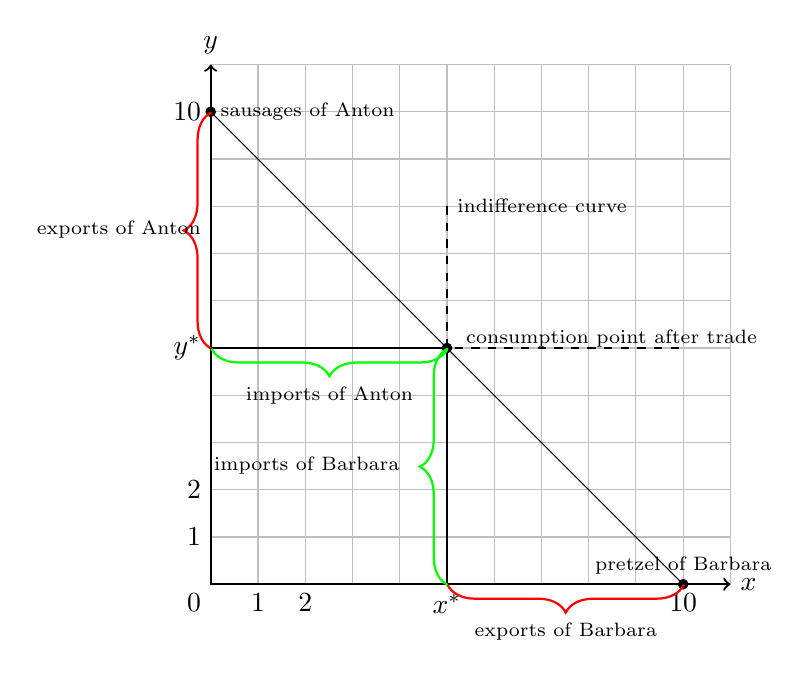
\begin{tikzpicture}[scale=0.6]
			\draw [color=gray!50]  [step=10mm] (0,0) grid (11,11);
			\draw[thick,<->] (0,11) node[above]{$y$}--(0,0)--(11,0) node[right]{$x$};
			\node [below left] at (0,0) {$0$};
			\node [below] at (5,0) {$x^{*}$};
			\node [below] at (1,0) {1};
			\node [below] at (2,0) {2};
			\node [below] at (10,0) {10};
%			\node [right] at (5,5) {optimal consumption point};
			\draw [fill] (5,5) circle [radius=.1] ;
			\node [right] at (5.2,5.2) {\scriptsize  consumption point after trade};
			\draw [fill] (0,10) circle [radius=.1] node[right]{\scriptsize sausages of Anton};
			\draw [fill] (10,0) circle [radius=.1] node[above]{\scriptsize pretzel of Barbara};
			\node [left] at (0,1) {1};
			\node [left] at (0,2) {2};
			\node [left] at (0,10) {10};
			\node [left] at (0,5) {$y^{*}$};
			\draw(0,10)--(10,0);
%			\node [right] at (10,.5) {$p_xx+p_yy=I$};
			\draw(0,5)--(5,5)--(5,0);
			\draw[thick,dashed] (5,8) node[right]{\scriptsize  indifference curve} --(5,5)--(10,5) ;
			\draw [thick, red,decorate,decoration={brace,amplitude=10pt,mirror},xshift=0.4pt,yshift=-0.4pt](5,0) -- (10,0) node[black,midway,yshift=-0.6cm] {\scriptsize  exports of Barbara};
			\draw [thick, green,decorate,decoration={brace,amplitude=10pt},xshift=0.4pt,yshift=-0.4pt](5,0) -- (5,5) ;
			\node [black, left] at (4.2,2.5) {\scriptsize  imports of Barbara} ; 
					
			\draw [thick, green,decorate,decoration={brace,amplitude=10pt,mirror},xshift=0.4pt,yshift=-0.4pt](0,5) -- (5,5) node[black,midway,yshift=-0.6cm] {\scriptsize  imports of Anton};
			\draw [thick, red,decorate,decoration={brace,amplitude=10pt},xshift=0.4pt,yshift=-0.4pt](0,5) -- (0,10) ;
			\node [black, left] at (0,7.5) {\scriptsize  exports of Anton} ; 
%			\draw(2,10) ..controls (3.33,6) and (6,3.33) .. (10,2) node[right]{$U(x,y)=U_0$};
		\end{tikzpicture}
	\end{center}

\pbn
d)

				\begin{center}
	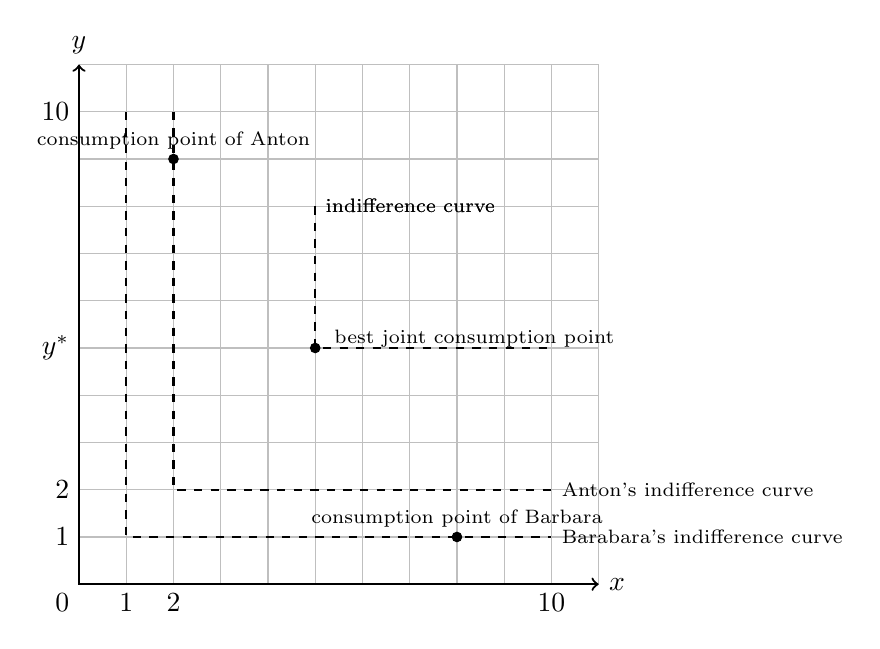
\begin{tikzpicture}[scale=0.6]
		\draw [color=gray!50]  [step=10mm] (0,0) grid (11,11);
		\draw[thick,<->] (0,11) node[above]{$y$}--(0,0)--(11,0) node[right]{$x$};
		\node [below left] at (0,0) {$0$};
%		\node [below] at (5,0) {$x^{*}$};
		\node [below] at (1,0) {1};
		\node [below] at (2,0) {2};
		\node [below] at (10,0) {10};
		%			\node [right] at (5,5) {optimal consumption point};
		\draw [fill] (2,9) circle [radius=.1] node[above]{\scriptsize consumption point of Anton} ;
		\draw [fill] (8,1) circle [radius=.1] node[above]{\scriptsize consumption point of Barbara} ;
%		\node [right] at (5.2,5.2) {\scriptsize  consumption point after trade};
%		\draw [fill] (0,10) circle [radius=.1] node[right]{\scriptsize sausages of Anton};
%		\draw [fill] (10,0) circle [radius=.1] node[above]{\scriptsize pretzel of Barbara};
		\node [left] at (0,1) {1};
		\node [left] at (0,2) {2};
		\node [left] at (0,10) {10};
		\node [left] at (0,5) {$y^{*}$};
%		\draw(0,10)--(10,0);
		\draw[thick,dashed] (2,10)  --(2,2)--(10,2) node[right]{\scriptsize  Anton's indifference curve} ;
		\draw[thick,dashed] (1,10)  --(1,1)--(10,1) node[right]{\scriptsize  Barabara's indifference curve} ;
		%			\node [right] at (10,.5) {$p_xx+p_yy=I$};
%		\draw(0,5)--(5,5)--(5,0);
		\draw [fill] (5,5) circle [radius=.1] ;
\node [right] at (5.2,5.2) {\scriptsize  best joint consumption point};
		\draw[thick,dashed] (5,8) node[right]{\scriptsize  indifference curve} --(5,5)--(10,5) ;
					\draw[thick,dashed] (5,8) node[right]{\scriptsize  indifference curve} --(5,5)--(10,5) ;
	\end{tikzpicture}
\end{center}
	}
	
	\pbn
	

	
	
	
	\subsection{Terms of trade}
	
	\boxb{
		The terms of trade is defined as the quantity of one good that exchanges for a quantity of another. In this case, how many apples can be exchanged for how many oranges? It is typical to express the terms of trade as a ratio. 
	}
	
	In the above example, the exchange of goods takes place at a ratio of 1:1. In economics, one speaks that the terms of trade are 1. The terms of trade is a ratio defined as the relative price of exports in relation to imports. In other words, the quantity of one good that can be exchanged for a quantity of another good. For example, how many sausages can be exchanged for how many pretzels.  The terms of trade, which are ultimately determined by the two trading partners, depend on a variety of different and distinct factors, including the following:
	
	\desx{
		\item[Preferences] For a trade to occur, each trader must desire something of the other good and be willing to give up something of his own good in order to obtain it. Put formally, the expected utility of eating a few slices of Anton's bread must be greater than the expected disutility of not eating a few of his sausages. The same logic applies to Barbara. In this case, extreme preferences were assumed. Normally, the two goods are not perfectly complementary, but substitutable.
		\item[Uncertainty]
		In this situation, both people have clearly defined preferences. Perhaps Barbara has never tried one of Anton's sausages, and Anton usually eats bread and not pretzels. A simple way to eliminate this uncertainty would be to offer free samples of their products before an exchange is agreed upon.  Without a sample, Anton and Barbara would have to make their exchanges based on their expectations of the taste of the other product. 	
		\item[Scarcity] The relative quantities of the two goods available for trade affect the terms of trade. Suppose consider pretzels and sausages not to be perfect complements and suppose Barbara has 1000 pretzels then the terms of trade would likely be different. 
		\item[Size]	
		The size of the goods is likely to affect the terms of trade. 
		\item[Quality] The quality of the goods will affect the terms of trade. Assuming the pretzels are old and hard, both individuals would likely prefer less than one pretzel per sausage.
		\item[Persuasion] If Barbara is a good salesperson and Anton is not, she may have the power to influence the terms of trade to her advantage.
		\item[Government Policy] Suppose a tax official is willing to impose a tax based on the quantities traded between Barbara and Anton, this is likely to influence the terms of trade. If the laws prohibit the two from meeting in person, they will not trade either. 
	} 
	
	\pbn
	\exextoc{Terms of trade}{
		\begin{center}
			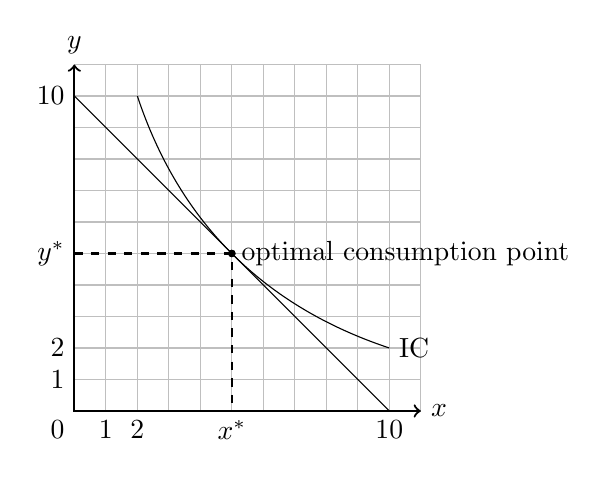
\begin{tikzpicture}[scale=0.4]
				\draw [color=gray!50]  [step=10mm] (0,0) grid (11,11);
				\draw[thick,<->] (0,11) node[above]{$y$}--(0,0)--(11,0) node[right]{$x$};
				\node [below left] at (0,0) {$0$};
				\node [below] at (5,0) {$x^{*}$};
				\node [below] at (1,0) {1};
				\node [below] at (2,0) {2};
				\node [below] at (10,0) {10};
				\node [left] at (0,1) {1};
				\node [left] at (0,2) {2};
				\node [left] at (0,10) {10};
				\draw [fill] (5,5) circle [radius=.1];
				\node [left] at (0,5) {$y^{*}$};
				\draw [fill] (5,5) circle [radius=.1];
				\node [right] at (5,5) {optimal consumption point};
				\draw(0,10)--(10,0);
				%			\node [right] at (10,.5) {$p_xx+p_yy=I$};
				\draw [thick,dashed] (0,5)--(5,5)--(5,0);
				\draw(2,10) ..controls (3.33,6) and (6,3.33) .. (10,2) node[right]{IC};
			\end{tikzpicture}
		\end{center}
		
		Suppose you have a fixed income $I=10$ that you can spend on consuming two substitutable goods $x, y$ at certain prices $p_x=1, p_y=1$. The current consumption decission is sketched in the figure above. Suppose the price of good $x$ increases, i.e., $p_x=2$. Draw the new budget line. How will consumption change? What are the new terms of trade?
	}
	
	\pbn
	\solx{Terms of trade}{
		The new point of optimal consumption $OCP_1$ at $(x=2,y=6)$ illustrates that an increase in the price of good $x$ leads consumers to substitute good $x$ and consume more of good $y$ but less of good $x$.\footnote{Please notice that the indifference curve $IC_1$ in the graph is just a guess of mine because we don't have preferences in form of a utility function given. For example, you can also draw an indifference curve that gives you the optimal consumption point at $(x= 1;y= 8)$ or $(x= 4;y= 2)$.} 
	The terms of trade are now $\frac{p_x}{p_y}=2$. That is, consumers are willing to give up 1 unit of good $x$ to receive 2 units of good $y$. The budget line is drawn in blue.
		
		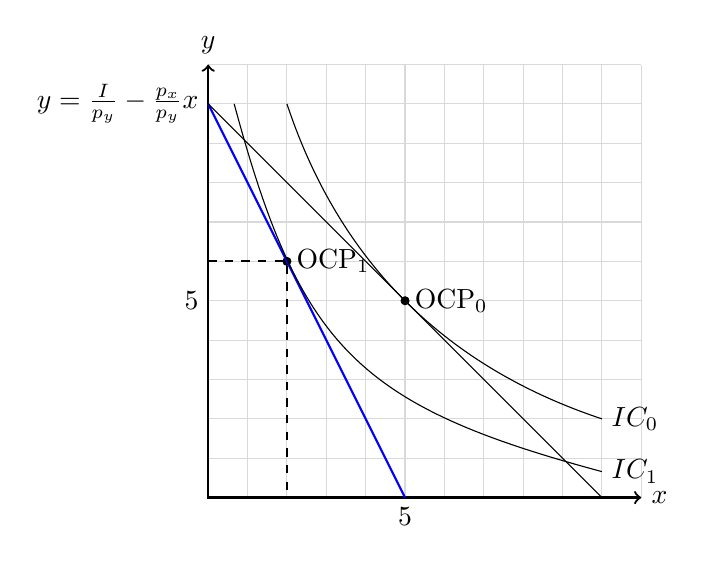
\begin{tikzpicture}[scale=0.5]
			\draw [color=gray!30]  [step=10mm] (0,0) grid (11,11);
			\draw[thick,<->] (0,11) node[above]{$y$}--(0,0)--(11,0) node[right]{$x$};
			\draw[thick,dashed] (0,6)--(2,6)--(2,0);
			\draw [fill] (5,5) circle [radius=.1];
			\node [right] at (5,5) {OCP$_0$};
			\node [below] at (5,0) {5};	\node [left] at (0,5) {5};
			\draw [fill] (2,6) circle [radius=.1];
			\draw [thick, blue] (0,10)--(5,0);
			\node [right] at (2,6) {OCP$_1$};
			\node [left] at (0,10) {$y=\frac{I}{p_y}-\frac{p_x}{p_y}x$};
			\draw(0,10)--(10,0);
			%				\draw(0,2.5)--(5,5)--(5,0);
			\draw(0.66,10) ..controls (2.33,3.8) and (3.8,2.33) .. (10,0.66) node[right]{$IC_1$};
			%	\draw(1,10) ..controls (2.33,6) and (6,2.33) .. (10,1) node[right]{$IC_1$};
			\draw(2,10) ..controls (3.33,6) and (6,3.33) .. (10,2) node[right]{$IC_0$};
		\end{tikzpicture}
	}
	
	
	
	
	
	\pbn
	\subsection{Endowments in an exchange economy}
	
	
	Trade is a decision to give up something in order to receive something in return. If this decision is made of free will, it must improve the situation of both participants in the trade (but not necessarily that of all those who are not involved in the trade in question).		
	
	\subsubsection{Fixed production}
	\begin{figure}
		\begin{center}
			\includegraphics[width=.8\linewidth]{$HOME/Dropbox/hsf/pic/ie/tausch_1_pdf}
			\caption{Optimizing consumption through trade}\label{fig:tausch_1}
		\end{center}
	
	\end{figure}
	\itex{
		\item Suppose country H produces $\bar{x}^H_1$ of good 1 and $\bar{x}^H_2$ of good 2. In autarky, all goods produced are consumed. The autarkic consumption is represented in \autoref{fig:tausch_1}. We see that point A in autarky is indeed welfare maximizing with utility $W^H_A$. 
		\item Now suppose country H can trade with other countries at world prices \[\left(\frac{p_1}{p_2}\right)_W>\left(\frac{p_1}{p_2}\right)_A,\] where $\left(\frac{p_1}{p_2}\right)_A$ denotes the price relation of country H in autarky.
		\item Then country H can use a consumption basket with a higher utility, $W_T^H>W_A^H$.
		\item This utility improvement is possible by exporting good $x_1$ and importing good $x_2$.
	}
	
	\pbn	
	\subsubsection{Flexible production}
	\begin{figure}
		\begin{center}
			\includegraphics[width=.7\linewidth]{$HOME/Dropbox/hsf/pic/ie/tausch_2_pdf}
			\caption{Optimizing consumption by adjusting production and trade }\label{fig:tausch_2}
		\end{center}
	
	\end{figure}
	\itex{	
		\item Trade is even more beneficial to a country if it can adjust its production to export more goods that are relatively high priced in the world market. This statement is shown in \autoref{fig:tausch_2}. 
		\item In autarky, optimal consumption would be at point A and optimal consumption would be at point C under free trade. Now suppose that producers in country H know that they can sell their goods at price $p_1^W$ and $p_2^W$ before deciding what to produce. Then they would choose production point B on the production frontier curve to export good $x_1$ and import good $x_2$ at price $\left(\frac{p_1}{p_2}\right)_A$ to be consumed at point D. Welfare at point D is higher than at point C or A because we end up at the highest indifference curve.			
	}
	
	\pbn
	\exextoc{Production and consumption}{
		The figure below shows the production possibility frontier curve, $PPF$, of a country, $H$, in autarky in which only two products, $x_1$ and $x_2$, can be produced and consumed, respectively. 
		\begin{center}
			\begin{tikzpicture}[scale=1.0]
				\draw [<-] (0,7.8) node [left] {$x_2$} -- (0,0);
				\draw [->] (0,0) -- (8.9,0) node [below] {$x_1$};
				\node [left] at (0,6.45) {$PPF$};
				\node [below] at (5.05,0) {$PPF$};
				%	\node [left] at (4.3,3.2) {$A$};
				node [below] at (2.4,5.4) {};
				
				\draw (5.8,.5) -- (2.65,6.7);
				%	\node [right] at (2.0,5.4) {$B$};
				%	\node [right] at (7.6,1.5) {$F$};
				%	\node [right] at (7.65,2.15) {$G$};
				\node [right] at (7.3,1.0) {$IC_{autarky}$};
				\node [right] at (5.65,.30) {$P_{autarky}$};
				\draw[fill] (4.37,3.3) circle [radius=0.06];
				%	\draw (.5,7.2) -- (7.7,1.7);
				%	\node [right] at (5.75,3.4) {$D$};
				%	\draw (4.45,5.3) to [out=-90, in=140] (5.75,3.2) to [out=-40, in=160] (7.7,2.2);
				\draw (4.1,4.6) to [out=-77, in=120] (4.54,3) to [out=-60, in=160] (7.4,1.1);
				\draw (0,6.45) to [out=0, in=115] (4.41,3.2) to [out=-65, in=90] (5.05,0);
			\end{tikzpicture}
		\end{center}
		\abcx{
			\item  Given the country is in autarky (i.e., no trade), the price relation of both goods within the country is represented by the line denoted with $P_{autarky}$. The indifference curve that represents the utility maximizing level of utility is denoted with $IC_{autarky}$. Mark in the figure how much of both goods are produced and consumed, respectively.  
			%	\part Explain briefly what the curve $B$ and line $C$ represent in the figure.
			\item Suppose country $H$ opens up to trade with foreign countries. Further assume that the country can trade with other countries at fixed world market prices  \[\left(\frac{p_1}{p_2}\right)_W>\left(\frac{p_1}{p_2}\right)_A,\]  where $\left(\frac{p_1}{p_2}\right)_A$ denotes the price relation of country H in autarky, $P_{autarky}$.
			Sketch the world market price relation in the figure and mark the new production point on the production possibility frontier curve. Moreover, mark below those statements that are \textbf{true}:
			\begin{enumerate}[i)] 
				\item Country $H$ will produce more of good $x_1$ than in autarky 
				\item  Country $H$ will produce more of good $x_2$ than in autarky
				\item Country $H$ will consume more of good $x_1$ than in autarky
				\item Country $H$ will export good $x_1$ and import good $x_2$.
				\item Country $H$ will export good $x_2$ and import good $x_1$.
				\item  Country $H$ will suffer a loss of welfare due to opening up to trade.
			\end{enumerate}	
		}
	}
	
	
	\pbn
	\exextoc{Gains of small economies}{
		Show that opening markets to foreign trade can be beneficial for a small economy where only two goods can be produced and consumed. Use a two-way diagram to do this. In particular, show the consumption and production point of the economy in autarky with the corresponding price relation. Then assume that the economy opens up to the foreign market, allowing it to buy goods at world prices that are different from prices in autarky. Show the consumption and production point of the autarkic economy with the corresponding price relation under free trade. Can you outline the higher level of welfare in free trade?
	}
	
	\pbn
	\solx{Gains of small economies}{
		The indifference curve under free trade lies above the IC under autarky. This reflects the higher utility level under free trade.
		\begin{center}
			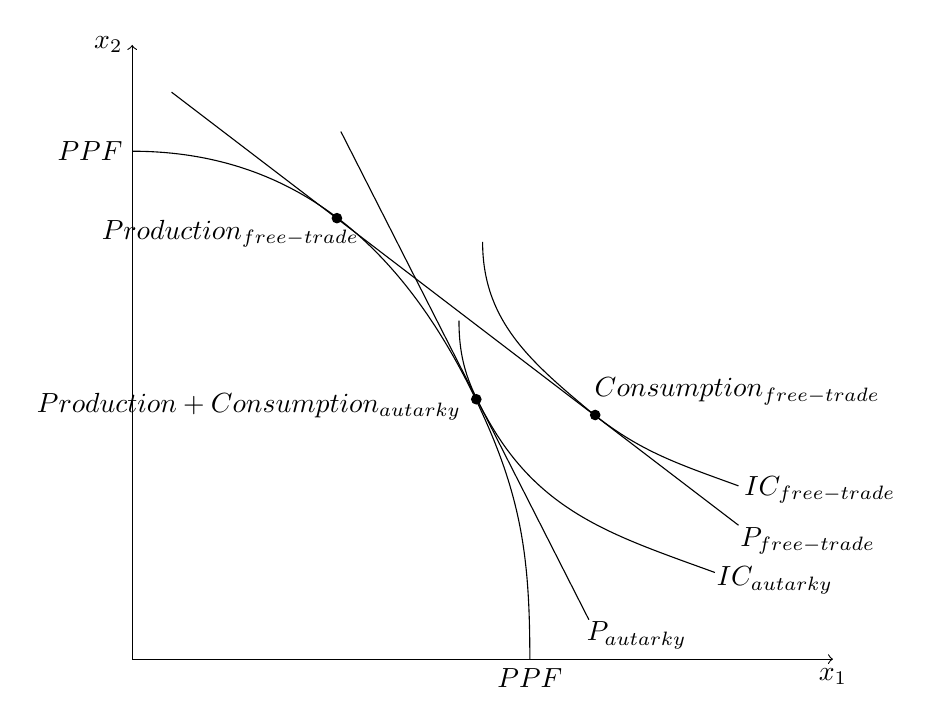
\begin{tikzpicture}[scale=1]
				\draw [<-] (0,7.8) node [left] {$x_2$} -- (0,0);
				\draw [->] (0,0) -- (8.9,0) node [below] {$x_1$};
				\node [left] at (0,6.45) {$PPF$};
				\node [below] at (5.05,0) {$PPF$};
				\node [left] at (4.3,3.2) {$Production+Consumption_{autarky}$};
				%	node [below] at (2.4,5.4) {};
				
				\draw (5.8,.5) -- (2.65,6.7);
				\node [left] at (3.0,5.4) {$Production_{free-trade}$};
				\draw[fill] (2.6,5.6) circle [radius=0.06];
				\node [right] at (7.6,1.5) {$P_{free-trade}$};
				\node [right] at (7.65,2.15) {$IC_{free-trade}$};
				\node [right] at (7.3,1.0) {$IC_{autarky}$};
				\node [right] at (5.65,.30) {$P_{autarky}$};
				\draw[fill] (4.37,3.3) circle [radius=0.06];
				\draw (.5,7.2) -- (7.7,1.7);
				\node [right] at (5.75,3.4) {$Consumption_{free-trade}$};
				\draw[fill] (5.88,3.1) circle [radius=0.06];
				\draw (4.45,5.3) to [out=-90, in=140] (5.75,3.2) to [out=-40, in=160] (7.7,2.2);
				\draw (4.15,4.3) to [out=-90, in=120] (4.54,3) to [out=-60, in=160] (7.4,1.1);
				\draw (0,6.45) to [out=0, in=115] (4.41,3.2) to [out=-65, in=90] (5.05,0);
			\end{tikzpicture}
		\end{center}
	}
	
	
	\pbn
	\section{More trade is not necessarily good (immiserizing growth)}\label{sec:imi}
	\itex{
		\item So far, I have implicitly assumed that the world market price is fixed and not changed by the entry of country H into the free trade market. When the latter is the case, economists speak of a small open economy (SOE). In general, a SOE is an economy that is so small that its policies do not change world prices. 
		\item Suppose that country H is not an SOE. What would happen to world prices if country H offered a lot of good $x_1$ to receive good $x_2$? Obviously, $\left(\frac{p_1}{p_2}\right)_W$ would fall. In the worst case, country H is so large that $\left(\frac{p_1}{p_2}\right)_W=\left(\frac{p_1}{p_2}\right)_A$. This means that country H has no benefits from free trade.
		\item Assuming that a (large) country cannot opt out from free trade and that the exporting sector grows, there is a theoretical scenario called \textit{immiserizing growth} that shows that free trade countries are worse off in the long run. This scenario is illustrated in \autoref{fig:immigrow}. The figure summarizes two periods. In the first period, country H produces at point B and consumes at point D, trading goods at world prices $\left(\frac{p_1}{p_2}\right)_W$. Then country H grows in sector 1. This is shown in the new production possibility curve TK2. If country H were able to trade at the old world price, it would be able to consume at point F. Unfortunately, country H is not a SOE, and therefore world prices (from country H's perspective) deteriorate to $\left(\frac{p_1}{p_2}\right)_W'$. This has bad implications for country H, since its optimal consumption is now at point D', which has lower welfare relative to point D. However, this is not an argument against trade, since the welfare at point D' is still above the production possibility curve in autarky, TK1. 
	}
	\begin{figure}
		\begin{center}
			\includegraphics[width=.7\linewidth]{$HOME/Dropbox/hsf/pic/ie/immigrow_pdf}
			\caption{Immiserizing growth }\label{fig:immigrow}
		\end{center}
	\end{figure}
	
	%
	%\exex{Gains through trade}{
	%The consumers' utility function in country H and F is $U=x_1\cdot x_2$ and the fixed production of both countries are $\bar{x}_1^H=\bar{x}_2^H=100$, $\bar{x}_1^F=500$ and $\bar{x}_2^F=100$.
	%\enxx{a)}{
	%	\item Calculate the demand function of both countries.
	%	\item Calculate the relative prices in autarky for both countries.
	%	\item Calculate the utility of both countries in autarky.
	%	\item Calculate the relative prices under free trade.
	%	\item Calculate the exports and imports of both countries.
	%	\item Calculate the utility of both countries under free trade.
	%	\item Draw a plot that shows the consumption points in autarky and under free trade.
	%	}
	%}
	%
	%
	%\begin{shadedbox}
	%	Please watch the video available on ILIAS, see: \url{Gains-through-trade }
	%\end{shadedbox}	
	%
	%\newpage
	%\solx{Gains through trade}{
	%	\enxx{a)}{
	%		\item Solving the Lagrangian multiplier,  $\mathcal{L}(x_1,x_2,\lambda)=x_1x_2-\lambda(p_1x_1+p_2x_2-I)$, we get $x_2p_2=x_1p_1$. Plugging this into the budget restriction $p_1x_1+p_2x_2=I$ and solving for $x_1$ and $x_2$ respectively, we get: 
	%		\begin{align*}
	%			x_1^*=\frac{I}{2}\cdot \frac{1}{p_1}\\
	%			x_2^*=\frac{I}{2}\cdot \frac{1}{p_2}
	%		\end{align*}
	%		\item In autarky the supply of goods is given by production. The relative prices adjust till demand equals supply:
	%		\begin{align*}
	%			\left(\frac{p_2}{p_1}\right)_H=1\\
	%			\left(\frac{p_2}{p_1}\right)_F=5
	%		\end{align*}
	%		\item 
	%		\begin{align*}
	%			U_H^A=100\cdot 100= 10000\\
	%			U_F^A=100\cdot 500= 50000\\
	%		\end{align*}
	%		\item Under free trade the supply of goods is given by production of both countries. The relative prices adjust till demand equals supply:
	%		\begin{align*}
	%		\frac{x_1}{x_2}=\left(\frac{p_2}{p_1}\right)_W=\frac{600}{200}=3
	%		\end{align*}
	%		\item Under free trade the value of exports of one country equals the value of the imports of the other country. We know that country H will import good 1 and export good 2. 
	%		\begin{align*}
	%			\underbrace{(\bar{x}_2^H-x_2)p_2}_{\textnormal{value of exports}}&= \underbrace{(x_1-\bar{x}_1^H)p_1}_{\textnormal{value of imports}}\\
	%			\Leftrightarrow (100-x_2)3 &=1(x_1-100)
	%		\end{align*}
	%		Using the demand relation, $\frac{x_1}{x_2}=3\Leftrightarrow x_1=3 x_2$, we get 
	%		\begin{align*}
	%			x_2^*&=\frac{200}{3}\\
	%			x_1^*&=200
	%		\end{align*}
	%		Thus, country H exports $\frac{100}{3}$ units of good 2 and imports 100 units of good 1, whereas F imports $\frac{100}{3}$ units of good 2 and exports 100 units of good 1.
	%		
	%		\item 
	%		\begin{align*}
	%			U_H^W=&200\cdot \frac{200}{3}= 13333 \frac{1}{3}\\
	%			U_F^W=&400\cdot \frac{400}{3}= 53333\frac{1}{3}
	%		\end{align*}
	%		Since $U_H^A<U_H^W$ and $U_F^A<U_F^W$, both countries increase their utility through free trade. 
	%		\item The following figure shows the consumption under autarky and free trade. The change in consumption through trade is marked with a blue arrow and the world market prices are drawn with dashed red lines.
	%	}
	%		 \begin{centering}
	%			\begin{tikzpicture}[scale=.7]
	%%			[yscale=.5,xscale=1.9]
	%			\draw [color=gray!50]  [step=10mm] (0,0) grid (6,9);
	%			\draw[thick,<->] (0,9) node[left]{$x_1$}--(0,0)--(6,0) node[right]{$x_2$};
	%			\draw[blue, thick,->] (1,1) --(2/3,2); 
	%			\draw[blue, thick,->] (1,5) --(4/3,4); 
	%			\node [below left] at (0,0) {$ $};%Origin
	%			\draw[red, dashed]  (0,4)   -- (4/3,0)  ;
	%			\draw[red, dashed]  (0,8)   -- (8/3,0)   ;
	%			\tkzDefPoint(1,1){A}
	%			\tkzLabelPoint[right,font=\tiny](A){(100,100)}
	%			\tkzDefPoint(1,5){B}
	%			\tkzLabelPoint[right,font=\tiny](B){(500,100)}
	%			\tkzDefPoint(2/3,2){C}
	%			\tkzLabelPoint[right,font=\tiny](C){(200,$\frac{200}{3}$)}
	%			\tkzDefPoint(4/3,4){D}
	%			\tkzLabelPoint[right,font=\tiny](D){(400,$\frac{400}{3}$)}
	%			\foreach \n in {B,A,C,D}
	%			\node at (\n)[circle,fill,inner sep=1.5pt]{};
	%			%	\draw[dotted] (0,0)--(4,4) node[left]{$x=y$};
	%			\end{tikzpicture}
	%			\captionof{figure}{Changes in consumption}\label{fig:cic}\end{centering}
	%}
	
	
	
	%%%%%%%%%%%%%%%%%%%%%%%%%%%%%%%%%%%%%%%%%%%% weiter gehts hier....................
	
	\section{The theory of comparative advantage (Ricardian Model)}\label{sec:ricardo}
	
	\boxx{\subsubsection*{Learning goals}
		%	After this part of the lecture, you will be able to:
		\itex{
			\item Less-developed
countries can compete in international markets even if they are less productive in producing everything. In other words, opening to trade is beneficial for countries that have an absolute disadvantage in the production of all goods.

			\item Both, developed and less-developed countries can gain from international trade.
			\item Specialization in production increases the price of exported goods for that country. As a result, prices converge. 
			\item A discussion of national competitiveness is not useful through the lens of the Ricardo theorem.
	}
\subsubsection{Recommended reading}
\itex{\item Chapter 2 of \bibentry{Academy2012International}}
}
	
	\begin{minipage}{0.4\linewidth}
		\begin{center}
			\includegraphics[width=0.7\linewidth]{../../../pic/ricardo}
		\end{center}
		\note{This painting shows Ricardo, aged 49 in 1821. Source: National Portrait Gallery}
	\end{minipage}
	\begin{minipage}{0.6\linewidth}
		\textbf{David Ricardo} (1772-1823), one of the most influential economists of his time, had a simple idea that had a major impact on how we think about trade. In \cite{Ricardo1819}, he argued that bilateral trade can be a positive-sum game for both countries, even if one country is less productive in all sectors, if each country specializes in what it can produce relatively best. 
		
		He introduced the theory of comparative advantage that is still an important corner stone of the modern theory of international trade\footnote{Actually, strictly speaking, this is not correct, since the original description of the idea can already be found in 1815 in the \textit{Essay on the External Corn Trade} by Robert Torrens. However, David Ricardo formalized the idea in his 1817 book using a convincing and simple numerical example. For more information on this, as well as a great introduction to the Ricardian model and more, I recommend \cite{Academy2012International}.} It refers to the ability of one party (an individual, a firm, or a country) to produce a particular good or service at a lower opportunity cost than another party. In other words, it is the ability to produce a product with the highest relative efficiency, given all other products that could be produced. In contrast, an absolute advantage is defined as the ability of one party to produce a particular good at a lower absolute cost than another party.
	\end{minipage}
	
\subsection{Defining absolute and comparative advantages}

A subject (country, household, individual, company) has an \textbf{absolute advantage} in the production of a good relative to another subject if it can produce the good at lower total costs or with higher productivity. Thus, absolute advantage compares productivity across subjects but within an item.

A subject has a \textbf{comparative advantage} in the production of a good relative to another subject if it can produce that good at a lower opportunity cost relative to another subject. 

	Let me explain the idea of the concept of comparative advantage with some examples:
	\paragraph{Old and young}
	Two women live alone on a deserted island. In order to survive, they have to do some basic activities like fetching water, fishing and cooking. The first woman is young, strong and educated. The second is older, less agile and rather uneducated. Thus, the first woman is faster, better and more productive in all productive activities. So she has an absolute advantage in all areas. The second woman, in turn, has an absolute disadvantage in all areas. In some activities, the difference between the two is large; in others, it is small.
	The law of comparative advantage states that it is not in the interest of either of them to work in isolation: They can both benefit from specialization and exchange. If the two women divide the work, the younger woman should specialize in tasks where she is most productive (e.g., fishing), while the older woman should focus on tasks where her productivity is only slightly lower (e.g., cooking). Such an arrangement will increase overall production and benefit both.
	
	\paragraph{The lawyer's typist}
	The famous economist and Nobel laureate Paul Samuelson (1915-2009) provided another example in his well-received textbook of economics, as follows: Suppose that in a given city the best lawyer also happens to be the best secretary. 
	However, if the lawyer focuses on the task of being a lawyer, and instead of practicing both professions at the same time, hires a secretary, both the lawyer's and the secretary's performance would increase because it is more difficult to be a lawyer than a secretary.\footnote{In the first eight editions the example comprised a
		male lawyer who was better at typing than his female secretary, but who had a comparative
		advantage in practising law. In the ninth edition published 1973, both lawyer and secretary were assumed to
		be female \citep[see][]{Backhouse2019Paul} Unfortunately, women are still discriminated against in introductory economics textbooks \citep[see][]{Stevenson2018Representations}.}
	
	

	
	
	\subsection{Autarky: An example of two different persons}\label{sec:exampleAB}
	
Assume that A and B want to produce and consume $y$ and $x$ respectively. Because of the complementarity of the two goods, each must be consumed in combination with the other. The utility function of both persons is $U_{\{A;B\}}=min(x,y)$. Both persons work for 4 time units, i.e., their \textit{units of labor} are $L_A=L_B=4$. A needs 1 units of labor to produce one unit of good $y$ and 2 units of labor to produce one unit of good $x$. B needs $\frac{4}{10}=0.4$ units of labor to produce one unit of good $y$ or good $x$. Thus, their \textbf{labor input coefficients}, which measure the units of labor required by a subject to produce one unit of good, are $a^A_y=1, a^A_x=2, a^B_y=0.4, a^B_x=0.4$:
			\begin{center}
		\begin{tabular}{lcc}\toprule
			&\multicolumn{2}{c}{Person}\\\cmidrule{2-3}
		input coefficient ($a$)	&A &B\\		\midrule
			Good $y$ & 1 & 0.4 \\
			Good $x$ & 2 & 0.4 \\\bottomrule
		\end{tabular}
	\end{center}\medskip
%	Further assume the two persons aim to consume as much as possible of the two goods which are perfect complementary, i.e.,  That means, they want to consume the goods together in a bundle in a ratio 1:1 (like we do it with a left and a right shoe).

Spending all her time in the production of $y$, A can produce  $\frac{L_A}{a_y^A}=\frac{4}{1}=4$ units of $y$ and B can produce $\frac{L_B}{a_y^B}=\frac{4}{0.4}=10$ units of $y$.
Spending all her time in the production of $y$, A can produce  $\frac{L_A}{a_x^A}=\frac{4}{2}=2$ units of $x$and B can produce $\frac{L_B}{a_x^B}=\frac{4}{0.4}=10$ units of $x$.    
Knowing this, we can easily draw the production possibility frontier curves (PPF) of person A and B as shown in \autoref{fig:ppf}. 

%				\begin{center}
%		\begin{tabular}{lcc}\toprule
%			&\multicolumn{2}{c}{Person}\\\cmidrule{2-3}
%			Maximum production ($\frac{L}{a}$)	&A &B\\		\midrule
%			Good $y$ & 4 & 10 \\
%			Good $x$ & 2 & 10 \\\bottomrule
%		\end{tabular}
%	\end{center}\medskip

	
	\begin{centering}
		\begin{tikzpicture}[scale=.7]
			\draw[thick,<->] (0,11) node[left]{$y$}--(0,0)--(11,0) node[right]{$x$}; % Axis and Lable
			\node [below left] at (0,0) {$ $};%Origin
			\draw(2,0)--(0,4) node[right]{$PPF_A$};
			\draw(10,0)--(0,10) node[right]{$PPF_B$};
			\draw[dashed,thick,red] (0,0)--(10,10) node[right]{possible consumption path $x=y$};
			\node [below left] at (0,0) {$0$};%Origin
			\tkzDefPoint(0,10){by}
			\tkzDefPoint(10,0){bx}
			\tkzLabelPoint[left](by){$10$}
			\tkzLabelPoint[below](bx){$10$}
			\tkzDefPoint(4/3,4/3){A}
			\tkzDefPoint(5,5){B}
			\tkzDefPoint(0,4){ay}
			\tkzDefPoint(2,0){ax}
			\tkzLabelPoint[left](ay){$4$}
			\tkzLabelPoint[below](ax){$2$}
			%\tkzLabelPoint[left](B){$x,y$}
			\foreach \n in {A, B}
			\node at (\n)[circle,fill,inner sep=1.5pt]{};
			\draw [dotted] (0,4/3) node [left] {$y^*_A=4/3$} -- (4/3,4/3) -- (4/3,0) node [below] {$x^*_A$};
			\draw [dotted] (0,5) node [left] {$y^*_B=5$} -- (5,5) -- (5,0) node [below] {$x^*_B=5$};
			%	\draw[fill] (1,1) circle [radius=0.06]
			\draw [blue,dashed,thick]  (4/3,3) -- (4/3,4/3) -- (3,4/3) node[right] {$IC_A$};
			\draw [blue,dashed,thick]  (5,6.3) -- (5,5) -- (6.3,5) node[right] {$IC_B$};
		\end{tikzpicture}
		\captionof{figure}{The production possibility frontier in autarky}\label{fig:ppf}
	\end{centering}

In autarky, both person maximize their utility: Individual A can consume $\frac{4}{3}$ units of each good and individual B can consume $5$ units of each good. The respective indifference curves are drawn in dashed blue lines in Figure \ref{fig:ppf}.
	
	\pbn
	\exextoc{Indifference curves for perfect complementary goods}{
		\abcx{
			\item Name some real world examples of goods that are perfectly complementary.
			\item The blue dashed lines in \autoref{fig:ppf} represent the indifference curves of individual A and B. The upward sloping dashed black line is denoted with ``possible consumption path''. Explain, why is it not correct--in strict sense--to name it like that?
		}
	}

	
	
	
	\subsubsection{Can person A and B improve their maximum consumption with cooperation?}
	Let us assume the two persons come together and try to understand how they can improve by jointly deciding which goods they should produce. If we assume that both persons redistribute their joint production so that both have an incentive to share and trade, we can concentrate on the total production output. Their joint PPF curve can then be drawn in two ways: 
	\enux{
		\item Person A specializes in good $x$, then the joint production possibilities are presented in \autoref{fig:ppfx}. 
		\item Person A specializes in good $y$, then the joint production possibilities are presented in \autoref{fig:ppfy2}.
	}
	
	
	\begin{minipage}[t]{0.5\textwidth}
		\begin{centering}
			\begin{tikzpicture}[scale=.4]
				\draw[thick,<->] (0,15) node[left]{$y$}--(0,0)--(14,0) node[right]{$x$}; 
				\draw[dashed] (0,0)--(10,10) node[left]{$x=y$};
				\node [below left] at (0,0) {$0$};%Origin
				\draw(2,10)--(0,14) node[right]{ };
				\draw(12,0)--(2,10) node[right]{$PPF^{\textnormal{world}}_{A\rightarrow x}$};
				\tkzDefPoint(0,14){by}
				\tkzDefPoint(0,10){by2}
				\tkzDefPoint(12,0){bx}
				\tkzDefPoint(2,0){bx2}
				\tkzLabelPoint[left](by){$14$}
				\tkzLabelPoint[left](by2){$10$}
				\tkzLabelPoint[below](bx){$12$}
				\tkzLabelPoint[below](bx2){$2$}
				\tkzDefPoint(7,7){py}
				\tkzDefPoint(6,6){px}
				\foreach \n in {px,py}
				\node at (\n)[circle,fill,inner sep=1.5pt]{};
				%	\draw [dotted] (0,6) node [left] {$y^*_B=6$} -- (6,6) -- (6,0) node [below] {$x^*_B=6$};
				\draw [dotted] (0,7) node [left] {$7$} -- (7,7) -- (7,0) node [below] {$7$};
				\draw [dotted] (0,6) node [left] {$6$} -- (6,6) -- (6,0) node [below] {$6$};
				%	\draw[fill] (1,1) circle [radius=0.06]
			\end{tikzpicture}
			\captionof{figure}{World PFF, A specializes in $x$}\label{fig:ppfx}\end{centering}
	\end{minipage}
	\begin{minipage}[t]{0.5\textwidth}
		\begin{centering}
			\begin{tikzpicture}[scale=.4]
				\draw[thick,<->] (0,15) node[left]{$y$}--(0,0)--(14,0) node[right]{$x$}; 
				\draw[dashed] (0,0)--(10,10) node[left]{$x=y$};
				\node [below left] at (0,0) {$0$};%Origin
				\draw(12,0)--(10,4) node[right]{$PPF^{\textnormal{world}}_{A\rightarrow y}$};
				\draw(10,4)--(0,14) node[right]{ };
				%	\draw[thick](2,10)--(0,14) ;
				%Koordinaten
				\coordinate (A) at (0,14);
				\coordinate (B) at (2,10);
				\coordinate (C) at (12,0);
				\coordinate (D) at (0,0);
				%	%Viereck - Füllung
				%	\fill[fill=black!30,opacity=0.2] (D) -- (A) -- (B) -- (C) -- cycle;
				%	\draw[thick](12,0)--(2,10) ;
				\tkzDefPoint(0,14){by}
				\tkzDefPoint(0,4){by2}
				\tkzDefPoint(12,0){bx}
				\tkzDefPoint(10,0){bx2}
				\tkzLabelPoint[left](by){$14$}
				\tkzLabelPoint[left](by2){$4$}
				\tkzLabelPoint[below](bx){$12$}
				\tkzLabelPoint[below](bx2){$10$}
				\tkzDefPoint(2,10){ppf}
				%	\tkzLabelPoint[below](ppf){$PPF_{A\rightarrow x}$}
				\tkzDefPoint(7,7){py}
				\tkzDefPoint(6,6){px}
				\tkzDefPoint(19/3,19/3){pa}
				%	\tkzLabelPoint[left](px){specialization of A in $x$}
				%	\tkzLabelPoint[left](pa){Autarky}
				\foreach \n in {px,py}
				\node at (\n)[circle,fill,inner sep=1.5pt]{};
				\draw [dotted] (0,7) node [left] {$7$} -- (7,7) -- (7,0) node [below] {$7$};
				\draw [dotted] (0,6) node [left] {$6$} -- (6,6) -- (6,0) node [below] {$6$};
			\end{tikzpicture}
			\captionof{figure}{World PFF, A specializes $y$}\label{fig:ppfy2}\end{centering}
	\end{minipage}
	
	
	
If A produces only good $x$, as shown in \autoref{fig:ppfx}, we see that A and B can consume a total of 6 units of goods $x$ and $y$. This is less in total than in autarky, where A can consume $\frac{4}{3}$ units of each good and person B can consume $5$ units of each good, giving a combined consumption of $\frac{19}{3}=6,\bar{6}$. 
	
If A produces only good $y$, as shown in \autoref{fig:ppfy2}, we see that A and B can consume a total of 7 units of goods $x$ and $y$. Thus, both can be better off compared to autarky, since the total quantity distributed is larger. Thus, we have an \textbf{Pareto improvement} here because at least one person can be better off compared to autarky.
	
\begin{figure}\centering
			\begin{tikzpicture}[scale=.6]
			\draw[thick,<->] (0,15) node[left]{$y$}--(0,0)--(14,0) node[right]{$x$}; 
			\draw[dashed] (0,0)--(10,10) node[left]{$x=y$};
			\node [below left] at (0,0) {$0$};%Origin
			\draw(12,0)--(10,4) node[right]{$PPF_{A\rightarrow y}$};
			\draw(10,4)--(0,14) node[right]{ };
			\draw[dotted](2,10)--(0,14) ;
			%Koordinaten
			\coordinate (A) at (0,14);
			\coordinate (B) at (2,10);
			\coordinate (C) at (12,0);
			\coordinate (D) at (0,0);
			%	%Viereck - Füllung
			\fill[fill=black!30,opacity=0.2] (D) -- (A) -- (B) -- (C) -- cycle;
			%	   \draw [fill=yellow]	(0,10) -- (0,14) -- (2,10) ;
			%	   \draw [fill=yellow]	(2,10) -- (0,0) -- (0,0) -- (12,0) ;
			\draw[dotted](12,0)--(2,10) ;
			\tkzDefPoint(0,14){by}
			\tkzDefPoint(0,4){by2}
			\tkzDefPoint(12,0){bx}
			\tkzDefPoint(10,0){bx2}
			\tkzLabelPoint[left](by){$14$}
			\tkzLabelPoint[left](by2){$4$}
			\tkzLabelPoint[below](bx){$12$}
			\tkzLabelPoint[below](bx2){$10$}
			\tkzDefPoint(2,10){ppf}
			\tkzLabelPoint[below](ppf){$PPF_{A\rightarrow x}$}
			%\tkzDefPoint(4/3,4/3){A}
			%\tkzDefPoint(5,5){B}
			%\tkzDefPoint(0,4){ay}
			%\tkzDefPoint(2,0){ax}
			%\tkzLabelPoint[left](ay){$4$}
			%\tkzLabelPoint[below](ax){$2$}
			%\tkzLabelPoint[left](B){$x,y$}
			\tkzDefPoint(7,7){py}
			\tkzDefPoint(6,6){px}
			\tkzDefPoint(19/3,19/3){pa}
			\tkzLabelPoint[right](py){specialization of A in $y$}
			\tkzLabelPoint[right](px){specialization of A in $x$}
			\tkzLabelPoint[left](pa){Autarky}
			\foreach \n in {pa,px,py}
			\node at (\n)[circle,fill,inner sep=1.5pt]{};
			%\draw [dotted] (0,4/3) node [left] {$y^*_A=4/3$} -- (4/3,4/3) -- (4/3,0) node [below] {$x^*_A$};
			\draw [dotted] (0,7) node [left] {$7$} -- (7,7) -- (7,0) node [below] {$7$};
			\draw [dotted] (0,6) node [left] {$6$} -- (6,6) -- (6,0) node [below] {$6$};
			%	\draw[fill] (1,1) circle [radius=0.06]
		\end{tikzpicture}
		\caption{World PFF in autarky when A specialize in producing good $y$}\label{fig:ppfy}
	\end{figure}

In \autoref{fig:ppfy}, the three possible consumption scenarios are marked with a dot and the PPFs of person A specializing in the production of good $x$ ($PPF_{A\rightarrow x}$) or good $y$ ($PPF_{A\rightarrow y}$) are also drawn. 
The scenario with person A specializing in the production of good $y$ is the output maximizing solution.\footnote{Note that this is also true for any other utility function, since $PPF_{A\rightarrow y}$ is always above $PPF_{A\rightarrow x}$.}

\subsubsection{Optimal production in cooperation} In order to produce the most bundles of both goods, the optimal cooperative production is 
				\begin{center}
	\begin{tabular}{lcc}\toprule
		&\multicolumn{2}{c}{Person} \\\cmidrule{2-3}
		production in cooperation	&A &B \\		\midrule
		Good $y$ & 4 & 3\\
		Good $x$ & 0 & 7 \\\bottomrule
	\end{tabular}
\end{center}\medskip


\subsubsection{Check for absolute advantage}
Employing 10 units of labor B can produce more of both goods and hence has an absolute advantage in producing $x$ and $y$. Formally, we can proof this by comparing the input coefficients of both countries in each good: 
\begin{center}
	\begin{tabular}{lcccl}\toprule
		&\multicolumn{3}{c}{Person}&\\\cmidrule{2-4}
		absolute advantage	&A & &B& \\		\midrule
		Good $y$ & $a_y^A=1$ & > & $0.4=a_y^B$ & $\Rightarrow$ B has an absolute advantage in good $y$\\
		Good $x$ & $a_x^A=2$ & > & $0.4=a_x^B$ & $\Rightarrow$ B has an absolute advantage in good $x$ \\\bottomrule
	\end{tabular}
\end{center}\medskip

\subsubsection{Check for comparative advantage}
	The slope of the PPFs represent the \textit{marginal rate of transformation}, the terms of trade in autarky and the opportunity costs of a country. The opportunity costs are defined by how much of a good $x$ (or $y$) a person (or country) has to give up to get one more of good $y$ (or $x$). For example, A must give up $\frac{a_x^A}{a_y^A}=\frac{1}{2}=0.5$ of good $x$ to produce one more of good $y$. Thus, A's opportunity costs of producing one unit of $y$ is the production foregone, i.e., a half good $x$. 
	All opportunity costs of our example are:
	
	\begin{center}
		\begin{tabular}{lcc}\toprule
			&\multicolumn{2}{c}{Person}\\\cmidrule{2-3}
			opportunity costs of producing \dots	&A &B\\		\midrule
			\dots1 unit of good $y$: & $\frac{a_y^A}{a_x^A}=\frac{1}{2}=0.5$  (good x) & $\frac{a_y^B}{a_x^B}=\frac{0.4}{0.4}=1$ (good x) \\
			\dots1 unit of good $x$: & $\frac{a_x^A}{a_y^A}=\frac{2}{1}=2$  (good y) & $\frac{a_x^B}{a_y^B}=\frac{0.4}{0.4}=1$  (good y) \\\bottomrule
		\end{tabular}
	\end{center}\medskip
	
Person A has a comparative advantage in producing good $y$ since A must give up less of good $x$ to produce one unit more of good $y$ than person B must. 
In turn, Person B has a comparative advantage in producing good $x$ since B must give up less of good $y$ to produce one unit more of good $x$ than person B must give up of good $y$ to produce one unit more of good $x$. 
Thus, every person has a comparative advantage and if both would specialize in producing the good in which they have a comparative advantage and share their output they can improve their overall output as was shown in \autoref{fig:ppfy}. 


%To explain what this means, denote $a^i_j$ the units of labor required by subject $i \in \{A,B\}$ to produce one unit of good $j\in \{x,y\}$. Since A can produce at most 4 units of good $y$ and 2 units of good $x$, we know that 
%	\[
%	a^A_y=1<a^A_x=2.
%	\]
%	Suppose A works 4 hours to produce good $x$, then he can produce four units of good $y$: $L_A/a^A_x=4/1=4$. 
%	
%	\red{Moreover, we know that \label{err:abverwechselt}
%		\[
%		a^B_y=0.4=a^B_x=0.4
%		\]
%		because with 4 units of labor, person B can produce 10 units of both goods.}
%	That means, individual B is more productive than A in producing good $y$ because $a^A_y>a^B_y$ and in producing good $x$ because $a^A_x>a^B_x$. 
	
%	However, A has a \textbf{comparative advantage} because 
%	\[
%	\frac{a^B_y}{a^B_x} \neq \frac{a^A_y}{a^A_x}.
%	\]
%	In particular, A (B) has a comparative advantage in producing good $y$ ($x$) because the ratio of the amount of labor required to produce a unit of $y$ to the amount of labor required to produce a unit of $x$ is lower for A compared to B:
%	\begin{align*}
%		\frac{a^B_y}{a^B_x} &> \frac{a^A_y}{a^A_x}.
%	\end{align*}
%	
%	Assuming both persons have 4 units of labor $(L_A=L_B=4)$, the labor input relations of both countries must be like this in order to get the PPF curves shown in \autoref{fig:ppf}:
%	\begin{align*}
%		\frac{a^B_y}{a^B_x} &> \frac{a^A_y}{a^A_x}\Leftrightarrow
%		\frac{0.4}{0.4} > \frac{1}{2} \Leftrightarrow 1> \frac{1}{2}.
%	\end{align*}
	
An alternative and more direct way to see the comparative advantages of A and B, respectively, is by comparing the two input coefficients of A with the two input coefficients of B: 
	\begin{align*}
		\frac{a^A_y}{a^A_x} &\lesseqqgtr \frac{a^B_y}{a^B_x} \quad	\Rightarrow \quad \frac{1}{2} <\frac{0.4}{0.4}.
	\end{align*}
Thus, A has a comparative advantage in $y$ and B in $x$.

\heux{Comparative advantage: Definition}{Economic subjects (e.g., individuals, households, firms, countries) should specialize in the production of that good in which they have a comparative advantage, that is, the ability of an economic subject to carry out a particular economic activity (e.g., producing goods) at a lower opportunity cost than a trade partner. 
	
%Two ways to check for the comparative advantage:

%\textbf{1. Opportunity costs:}
%
%		\itex{
%		\item $\frac{a^A_y}{a^A_x} < \frac{a^B_y}{a^B_x} \Rightarrow$  country A (B) has a comparative advantage in good y (x)
%		\item $\frac{a^A_x}{a^A_y} < \frac{a^B_x}{a^B_y} \Rightarrow$  country A (B) has a comparative advantage in good x (y)
%		\item $\frac{a^A_y}{a^A_x} = \frac{a^B_y}{a^B_x} \Rightarrow$  no country has a comparative advantage 
%		\item $\frac{a^A_x}{a^A_y} = \frac{a^B_x}{a^B_y} \Rightarrow$  no country has a comparative advantage 
%	}
%
%\textbf{2. Input coefficients:}

	\itex{
		\item $\frac{a^A_y}{a^A_x} > \frac{a^B_y}{a^B_x} \Rightarrow$  country A (B) has a comparative advantage in good x (y)
		\item $\frac{a^A_y}{a^A_x} < \frac{a^B_y}{a^B_x} \Rightarrow$  country A (B) has a comparative advantage in good y (x)
		\item $\frac{a^A_y}{a^A_x} = \frac{a^B_y}{a^B_x} \Rightarrow$  no country has a comparative advantage 
}
}

%In \autoref{fig:ppfy} we showed that it is output maximizing when both countries specialize in the production where they have a comparative advantage.


\subsubsection{Trade structure and consumption in cooperation}
If A specializes in the production of $y$, she must import some of good $y$, otherwise she cannot consume a bundle of both goods as desired. In turn, B wants to import some of the good $y$. 
B will not accept to consume less than 5 bundles of $y$ and $x$ as this was his autarky consumption. Thus, B wants a minimum of 2 units of good $y$ from A. A will not accept to give more than $4-\frac{4}{3}=2\frac{2}{3}$ items of good $y$ away and he wants at least $\frac{4}{3}$ items of good $x$. Overall, we can define three trade scenarios:

1. All gains from cooperation goes to A (see \autoref{fig:1winner}):

\begin{minipage}[t]{0.4\textwidth}
	\begin{center}
		\begin{tabular}{lcc}\toprule
			&\multicolumn{2}{c}{Person} \\\cmidrule{2-3}
			consumption in cooperation	&A &B \\		\midrule
			Good $y$ & 2 & 5\\
			Good $x$ & 2 & 5 \\\bottomrule
		\end{tabular}
	\end{center}
\end{minipage}
\begin{minipage}[t]{0.59\textwidth}
	\begin{center}
		\begin{tabular}{lcc}\toprule
			Trade	&\multicolumn{2}{c}{Person} \\\cmidrule{2-3}
			inflow/outflow of goods in cooperation	&A &B \\		\midrule
			Good $y$ & -2 & 2\\
			Good $x$ & 2 & -2 \\\bottomrule
		\end{tabular}
	\end{center}
\end{minipage}

2. All gains from cooperation goes to B:

\begin{minipage}[t]{0.4\textwidth}
	\begin{center}
		\begin{tabular}{lcc}\toprule
			&\multicolumn{2}{c}{Person} \\\cmidrule{2-3}
			consumption in cooperation	&A &B \\		\midrule
			Good $y$ & $\frac{4}{3}$ & 5$\frac{2}{3}$\\
			Good $x$ & $\frac{4}{3}$ & 5$\frac{2}{3}$ \\\bottomrule
		\end{tabular}
	\end{center}
\end{minipage}
\begin{minipage}[t]{0.59\textwidth}
	\begin{center}
		\begin{tabular}{lcc}\toprule
			Trade	&\multicolumn{2}{c}{Person} \\\cmidrule{2-3}
			inflow/outflow of goods in cooperation	&A &B \\		\midrule
			Good $y$ & $-\frac{2}{3}$ & $\frac{2}{3}$\\
			Good $x$ & $\frac{4}{3}$ & $-\frac{4}{3}$ \\\bottomrule
		\end{tabular}
	\end{center}
\end{minipage}

3. The gains from specialization and trade are shared by A and B: Some trade structure between the two shown above.

Each of the three cases yield a pareto-improvement, i.e., none gets worst but at least one gets better by mutually decide on production and redistribute the joint output. In the real world, however, it is often difficult for countries to cooperate and decide mutually on production and consumption. In particular, it is practically difficult to enforce redistribution of the joint outcome so that everyone is better off. 
So let's examine whether there is a mechanism that yields trade gains for both trading partners.

%
%In the example of \autoref{sec:exampleAB}, person A specializes in production where it has a comparative advantage in good $y$. To gain from specialization, A must export. Suppose A can convert one unit of good $y$ into one unit of good $x$ on the world market (which is B here). These terms of trade are represented by the red line in \autoref{fig:1winner}. Then, A exports 2 units of good $y$ and receives 2 units of good $x$ in return. In the end, it can consume 2 units of both goods. Since country B now produces 7 units of good $x$ and 3 units of good $y$, but exports 2 units of good $y$ and imports 2 units of good $x$, it remains at the same consumption level of 5 goods compared to autarky. Thus, person B does not benefit from trade in this scenario and thus has no incentive to trade.

%\paragraph{Can a general rule be derived from this example?}  Yes, B does not benefit here because it is incompletely specialized and the relative world prices, $\frac{p_y}{p_x}=1$, are the same for country B in autarky and free trade. Therefore, country B cannot benefit from trade because its specialization in good $x$ does not yield efficiency surpluses.
%%	\footnote{This would change if we assumed increasing returns to production.

%\paragraph{How can B also win?} Country A would also win on other terms of trade if they lie somewhere between the domestic terms of trade $(\frac{p_x}{p_y}=-\frac{2}{1})$ and the domestic terms of trade B $(\frac{p_x}{p_y}=-1)$.\\ For example, $\frac{p_x}{p_y}=-1.00000001$ would bring both in a winning scenario. 

\begin{figure}\centering
	\begin{tikzpicture}[scale=.90]
		\draw[thick,<->] (0,11) node[left]{$y$}--(0,0)--(11,0) node[right]{$x$}; % Axis and Lable
		\node [below left] at (0,0) {$ $};%Origin
		%	\draw[red] (4/3,4/3)-- (4/3,2) node[right]{EX};
		\draw (2,0)--(0,4) node[right]{$ $};
		\draw[red](4,0) --(0,4) ;
		\node [red, right] at (4,0.5) {$\frac{p_x}{p_y}=-1$};
		\draw(10,0)--(0,10) node[right]{$PPF_B$};
		\draw[dashed] (0,0)--(10,10) node[left]{$x=y$};
		\node [below left] at (0,0) {$0$};%Origin
		\tkzDefPoint(0,10){by}
		\tkzDefPoint(10,0){bx}
		\tkzLabelPoint[left](by){$10$}
		\tkzLabelPoint[below](bx){$10$}
		\tkzDefPoint(4/3,4/3){A}
		\tkzDefPoint(5,5){B}
		\tkzLabelPoint[right,font=\scriptsize](B){$(5,5) \rightarrow $ Consumption}
		\tkzDefPoint(2,2){C}
		\tkzLabelPoint[right,font=\scriptsize](C){$(2,2) \rightarrow $ Consumption}
		\tkzDefPoint(7,3){D}
		\tkzLabelPoint[right,font=\scriptsize](D){$(7,3) \rightarrow $ Production}
		\tkzDefPoint(0,4){E}
		\tkzLabelPoint[right,font=\scriptsize](E){$(0,4) \rightarrow $ Production}
		\tkzDefPoint(0,4){ay}
		\tkzDefPoint(2,0){ax}
		\tkzDefPoint(4,0){ax2}
		\tkzLabelPoint[left](ay){$4$}
		\tkzLabelPoint[below](ax){$2$}
		\tkzLabelPoint[below](ax2){$4$}
		
		%\tkzLabelPoint[left](B){$x,y$}
		\foreach \n in {B, C, D, E}
		\node at (\n)[circle,fill,inner sep=1.5pt]{};
		%	\draw [dotted] (0,4/3) node [left] {$y^*_A=4/3$} -- (4/3,4/3) -- (4/3,0) node [below] {$x^*_A$};
		%	\draw [dotted] (0,5) node [left] {$y^*_B=5$} -- (5,5) -- (5,0) node [below] {$x^*_B=5$};
		%	\draw[fill] (1,1) circle [radius=0.06]
		%	\draw [decorate,decoration={brace,amplitude=4pt},xshift=-4pt,yshift=0pt]
		%	(-0.5,2) -- (-0.5,4.0) node [black,midway,xshift=-0.9cm] 
		%	{\scriptsize $\textnormal{Export}^x_{AB}$} ;
		\draw [decorate, decoration={brace,amplitude=5pt,raise=1pt}] (2,2) --  node [below=6pt,font=\tiny]{Import$_{A}$} (0,2);
		\draw [decorate, decoration={mirror,brace,amplitude=5pt,raise=1pt}] (0,4) --  node [left=6pt,font=\tiny]{Export$_{A}$}  (0,2) ;
		
		
		\draw [decorate, decoration={brace,mirror,amplitude=5pt,raise=1pt}] (5,3) --  node [below=6pt,font=\tiny]{Export$_{B}$} (7,3);
		\draw [decorate, decoration={brace,amplitude=5pt,raise=1pt}] (5,3) --  node [left=6pt,font=\tiny]{Import$_{B}$} (5,5);
	\end{tikzpicture}
	\caption{Bilateral trade with one winner}\label{fig:1winner}
\end{figure}

\pbn
\subsection{The Ricardian model}
	To understand the underlying logic of the argument, let us formalize and generalize the situation of two subjects and their choices for production and consumption. In particular, the Ricardian Model build on the following assumptions:
	\itex{
		\item 2 subjects (A,B) can produce 2 goods (x,y) with 
		\item technologies with constant returns to scale.  Moreover, 
		\item production limits are defined by \[a_y^i Q_y^i+ a_x^i Q_x^i=L^i, \]
		where $a^i_j$ denotes the unit of labor requirement for person $i \in \{A,B\}$ in the production of good $j\in \{x,y\}$ and $Q^i_j$ denotes the quantity of good $j$ produced by person $i$, and 
		$Q^i_j$ the quantity of good $j$ produced by person $i$ and $Q^i_j$ the quantity of good $j$ produced by person $i$. (Imagine they both work 4 hours).
		\item Let $a^i_j$ denote the so-called labor input coefficients, i.e., the units of labor required by a person $i \in \{A,B\}$ to produce one unit of good $j\in \{x,y\}$.
		\item Suppose further that person B requires fewer units of labor to produce both goods, i.e., $a^A_y>a^B_y$ and $a^A_x>a^B_x$, and that
		\item a comparative advantage exists, i.e., $\frac{a^B_y}{a^B_x} \neq \frac{a^A_y}{a^A_x}$. 
	}
	

	
	\pbn
	\heux{Ricardian theorem}{
		If each country specialize in the production in the good for which it has a comparative advantage and exports this good, both countries gain from trade when the new world market price relation, $\frac{p^*_y}{p^*_x}$, lies between the price relations of both countries\footnote{In order to see that the relative prices within a country equals the relative productivity parameters, consider that nominal income of labor in producing good $j\in \{x,y\}$, $w_jL^i_j$, must equal the production value, that is, $p_j^ix_j^i$: 
			\[
			w_jL^i_j=p_j^ix_j^i.
			\]
			Setting $w_j=1$ as the numeraire and re-arranging the equation, we get
			\[ 
			p_j^i=\frac{L_j^i}{x_j^i}=a_j^i.
			\]} 
		\begin{align*}
			\frac{a^B_y}{a^B_x}  = \frac{p^B_y}{p^B_x} &> \frac{a^*_y}{a^*_x}= \frac{p^*_y}{p^*_x}> \frac{p^A_y}{p^A_x} = \frac{a^A_y}{a^A_x}
		\end{align*}
		because the consumption possibilities enlarge for both countries compared to a situation with no trade.
	}
	
%	\pbn
%	\subsubsection{Important implications of the Ricardian theorem:}
%	\itex{
%
%	}
	
	\pbn
	\subsection{Distribution of welfare gains}
	The Ricardo theorem tells us nothing about the precise distribution of welfare gains. In this section, I will show that the distribution of welfare gains is the result of relative supply and demand in the world.
	
	To illustrate this, consider Ricardo's famous example\footnote{The example is explained by \citet{Academy2012International} in greater detail.} of two countries (England and Portugal) that can produce cloth $T$ and wine $W$ with different input requirements, namely:
	\begin{align*}
		\frac{p^P_W}{p^P_T}=\frac{a^P_W}{a^P_T}=\frac{8}{9}<\frac{12}{10}=\frac{a^E_W}{a^E_T}= \frac{p^E_W}{p^E_T}
	\end{align*}
	Thus, England has an absolute disadvantage in the production of both goods, but England has a \textit{comparative advantage in the production of cloth} and Portugal has a \textit{comparative advantage in the production of wine}. Let us further assume that both countries are similarly endowed with labor, $\bar{L}$. Then we can calculate the world supply of cloth and wine given relative world prices, $\frac{p_T}{p_W}$. Since we know that Portugal will only produce wine if the price of wine relative to cloth is above $\frac{p_W}{p_T}=\frac{8}{9}$ and England will only produce wine if the price of wine relative to cloth is above $\frac{p_W}{p_T}=\frac{12}{10}$, we can draw the relative world supply of goods as shown in the left panel of \autoref{fig:rica_dem1}. Note that $\alpha$ in the figure means $\frac{1}{a}$. Similarly, we can draw in the world supply of clothes, shown in the left panel of \autoref{fig:rica_dem1}.
	
	
	\begin{center}
		\includegraphics[width=.7\linewidth]{$HOME/Dropbox/hsf/pic/ie/rica_dem1_pdf}
		\captionof{figure}{World's relative supply}\label{fig:rica_dem1}\bigskip
	\end{center}
	
	Whether both countries specialize totally in the production of one good, or only one country does so depends on world demand for both goods at relative prices. Since we know from the Ricardo Theorem that the world market price relation, $\frac{p^{*}_T}{p^{*}_W}$, must be between the two autarky price relations:
	\[
	\frac{p^P_T}{p^P_W}>\frac{p^{*}_T}{p^{*}_W}> \frac{p^E_T}{p^E_W}.
	\]
	If world demand for cloth would be sufficiently high to have a world price of $\frac{p^P_T}{p^P_W}=\frac{9}{8}$ Portugal would not gain from trade. On the contrary, if world demand for wine would be sufficiently high to have a world price of $\frac{p^P_T}{p^P_W}=\frac{10}{12}$ England would not gain from trade. Thus, the price span between $\frac{10}{12}$ and $\frac{9}{8}$ says us which country gains from trade.  For example, at a world price of $\frac{p^{*}_T}{p^{*}_W}=1$ about 57\% 
	\red{$\left[\frac{\left(1-\frac{10}{12}\right)}{\left(\frac{9}{8}-\frac{10}{12}\right)}\approx 0.57 \right] $}
	of the gains through trade will be distributed to Portugal and about 43\% will be distributed to England.
	
	In \autoref{fig:rica_dem2}, I show two demand curves of the World. The dashed demand curve represents a world with a relative strong preference on wine and the other demand curve represents a relative strong demand for cloth. Since Portugal has a comparative advantage in producing wine, they would happy to live in a world where demand for wine is relatively high, whereas the opposite holds true for England.\bigskip
	
	\begin{center}
		\includegraphics[width=.8\linewidth]{$HOME/Dropbox/hsf/pic/ie/rica_dem2_pdf}
		\captionof{figure}{World's relative supply and demand}\label{fig:rica_dem2}\bigskip
	\end{center}
	

	
	\pbn
\exextoc{Comparative advantage and opportunity costs}{
	Assume that only two countries, A and B, exist. Both countries are equally endowed with labor which is the only production factor. Both countries can produce either good $y$ or good $x$. The table below gives the input coefficients, $a$, for both countries, i.e., the units of labor needed to produce one unit of good $y$ and good $x$, respectively. Assume that both countries have 12 units of labor available.
	
	\begin{center}
		\begin{tabular}{lcc}\toprule
			&\multicolumn{2}{c}{Countries}\\\cmidrule{2-3}
			&A &B\\		\midrule
			Good $y$ & 1 & 3 \\
			Good $x$ & 2 & 4 \\\bottomrule
		\end{tabular}
	\end{center}\medskip
	
	\abcx{
		\item Name the country with an absolute advantage.
		\item Draw the production possibility curves in a y-x-diagramm.
		\item What are \textit{opportunity costs}?
		\item Calculate how many goods of $x$ country A has to give up to produce one unit more of good $y$.
		\item Calculate how many goods of $y$ country A has to give up to produce one unit more of good $x$.
		\item Calculate how many goods of $x$ country B has to give up to produce one unit more of good $y$.
		\item Calculate how many goods of $y$ country B has to give up to produce one unit more of good $x$.
		\item Name the country with a comparative advantage in good $y$. 
		\item Name the country with a comparative advantage in good $x$.
	}
}

\pbn
\solx{Comparative advantage and opportunity costs}{
	\abcx{
		\item Country A has an absolute advantage in producing both goods as 
		$$
		a_y^A=1<3=a_y^B
		$$
		and 
		$$
			a_x^A=2<4=a_x^B
		$$
		\item Solution is shown in the lecture.
		\item Opportunity cost is the value of what you lose when choosing between two or more options. Alternative definition: Opportunity cost is the loss you take to make a gain, or the loss of one gain for another gain.
		\item If A wants top produce one unit more of good $y$ it has to give up $\frac{1}{2}$ units of good $x$.
		\item If A wants top produce one unit more of good $x$ it has to give up $2$ units of good $y$.
		\item If B wants top produce one unit more of good $y$ it has to give up $\frac{3}{4}$ units of good $x$.
		\item If A wants top produce one unit more of good $x$ it has to give up $\frac{4}{3}$ units of good $y$.
		
			\begin{center}
			\begin{tabular}{lcc}\toprule
				&\multicolumn{2}{c}{Person}\\\cmidrule{2-3}
				opportunity costs of producing \dots	&A &B\\		\midrule
				\dots1 unit of good $y$ & $\frac{a_y^A}{a_x^A}=\frac{1}{2}=0.5$  (good x) & $\frac{a_y^B}{a_x^B}=\frac{3}{4}$ (good x) \\
				\dots1 unit of good $x$ & $\frac{a_x^A}{a_y^A}=\frac{2}{1}=2$  (good y) & $\frac{a_x^B}{a_y^B}=\frac{4}{3}=$  (good y) \\\bottomrule
			\end{tabular}
		\end{center}\medskip

		\item 	Country A has a comparative advantage in producing good $y$.
		\item 	Country B has a comparative advantage in producing good $x$.\label{error:compxy}
	}
}

	\pbn
\exextoc{The best industry is not competitive}{
	Assume that only two countries, A and B, exist. Both countries are equally endowed with labor which is the only production factor. Both countries can produce either good $y$ or good $x$. The table below gives the input coefficients, $a$, for both countries, i.e., the units of labor needed to produce one unit of good $y$ and good $x$, respectively.
	
	\begin{center}
		\begin{tabular}{lcc}\toprule
			&\multicolumn{2}{c}{Countries}\\\cmidrule{2-3}
			&A &B\\		\midrule
			Good $y$ & 10 & 9 \\
			Good $x$ & 12 & 10 \\\bottomrule
		\end{tabular}
	\end{center}\medskip
	
	Discuss absolute and comparative advantages. How much faster does B needs to in producing good $y$ to become an exporter of that good?
}

\pbn
\solx{The best industry is not competitive}{
	B has an absolute advantage in both goods. The opportunity costs are given by:
				\begin{center}
		\begin{tabular}{lcc}\toprule
			&\multicolumn{2}{c}{Country}\\\cmidrule{2-3}
			opportunity costs of producing \dots	&A &B\\		\midrule
			\dots1 unit of good: $y$ &  $\frac{a_x^A}{a_y^A}=\frac{10}{12}= 0.833\dots $ (good x) & $\frac{a_y^B}{a_x^B}=\frac{9}{10}=0.9$  (good x) \\			
			\dots1 unit of good: $x$ & $\frac{a_y^A}{a_x^A}=\frac{12}{10}=1.2$ (good y) & $\frac{a_x^B}{a_y^B}=\frac{10}{9} = 1.11\dots$ (good y) \\\bottomrule
		\end{tabular}
	\end{center}\medskip
Thus, A has a comparative advantage in producing good $y$ and B has a comparative advantage in producing good $x$. This seems to be counterintuitive as B can produce faster anything and everybody else. 

When looking on input coefficients, we get
$$
\frac{a^A_y}{a^A_x}=\frac{10}{12} < \frac{9}{10}=\frac{a^B_y}{a^B_x}
$$
which gives us the same comparative advantages as described above.

To become an exporter of $y$, B needs to have lower opportunity costs in the production of $y$ than A. This can happen by becoming more productive in producing $y$ \textbf{and/or} by becoming 'slower' in producing good $x$ so that  $\frac{a_y^B}{a_x^B}<\frac{10}{12}$
}

	\pbn
\exextoc{Comparative advantage and input coefficients}{
	Assume that only two countries, A and B, exist. Both countries are equally endowed with labor which is the only production factor. Both countries can produce either good $y$ or good $x$. The table below gives the input coefficients, $a$, for both countries, i.e., the units of labor needed to produce one unit of good $y$ and good $x$, respectively.
	
	\begin{center}
		\begin{tabular}{lcc}\toprule
			&\multicolumn{2}{c}{Countries}\\\cmidrule{2-3}
			&A &B\\		\midrule
			Good $y$ & 400 & 2 \\
			Good $x$ & 300 & 1 \\\bottomrule
		\end{tabular}
	\end{center}\medskip
	
	\abcx{
		\item Name the country with an absolute advantage.
		\item Name the country with a comparative advantage in good $y$. 
		\item Name the country with a comparative advantage in good $x$.
	}
}

\pbn
\solx{Comparative advantage and input coefficients}{
	\abcx{
		\item 	Country B has an absolute advantage in producing both goods.
		\item 	Country A has a comparative advantage in producing good $y$.
		\item 	Country B has a comparative advantage in producing good $x$.\label{error:compxy}
	}
}
	
	\pbn
	\exextoc{Comparative advantage: Germany and Bangladesh}{
		The table below gives the unit of labor needed to produce one machine, one ship, and one cloth in Germany and Bangladesh.
		
		\begin{center}
			\begin{tabular}{lccc}\toprule
				&Machine & Ship & Cloth\\\midrule
				Bangladesh & 100 & 10000 & 50\\
				Germany & 5 & 50  & 3 \\\bottomrule
			\end{tabular}
		\end{center}\medskip
		
		\enxx{a)}{
			\item Which country has an absolute advantage in the production of machines, ships, and clothes?
			\item What is  Germany's and Bangladesh's comparative advantage if we look only at machines and ships?
			\item What is  Germany's and Bangladesh's comparative advantage if we look only at machines and clothes?
			\item What is  Germany's and Bangladesh's comparative advantage if we look only at ships and clothes?
			\item Can you infer from the previous calculations which good Germany will
			export for sure and which good it will surely not export?
		}
	}
	
	\pbn
	\solx{Comparative advantage: Germany and Bangladesh}{
		\enxx{a)}{
			\item Germany has an absolute advantage in the production of the three goods because it labor input coefficients are smaller in all three goods.
			\item Since $p^{m/s}_B=\frac{100}{10000}<p^{m/s}_G=\frac{5}{50}$ Bangladesh has a comparative advantage in producing machines and Germany has a comparative advantage in producing ships.
			\item Since $p^{m/c}_B=\frac{100}{50}>p^{m/c}_G=\frac{5}{3}$ Bangladesh has a comparative advantage in producing clothes and Germany has a comparative advantage in producing machines.
			\item Since $p^{s/c}_B=\frac{10000}{50}>p^{s/c}_G=\frac{50}{3}$ Bangladesh has a comparative advantage in producing clothes and Germany has a comparative advantage in producing ships.
			\item Germany has a clear comparative advantage in producing ships and hence will export ships. Moreover, Germany has a clear comparative disadvantage in producing cloth and will definitely import clothes.
		}
	}
	
	\pbn
	\exextoc{Multiple choice: Ricardian model}{Assume that only two countries, A and B, exist. Both countries are equally endowed with labor which is the only production factor. Both countries can produce either good $y$ or good $x$. The table below gives the input coefficients, $a$, for both countries, i.e., the units of labor needed to produce one unit of good $y$ and good $x$, respectively.
		
		\begin{center}
			\begin{tabular}{lcc}\toprule
				&\multicolumn{2}{c}{Countries}\\\cmidrule{2-3}
				&A &B\\		\midrule
				Good $y$ & 40 & 20\\
				Good $x$ & 30 & 10 \\\bottomrule
			\end{tabular}
		\end{center}\medskip
		
		Which of the following statements is/are true? 
		\abcx{\item Country A has an absolute advantage in producing both goods.
			\item Country B has an absolute advantage in producing both goods.
			\item Country A has a comparative advantage in good $y$ and a comparative disadvantage in good $x$.
			\item Country B has a comparative advantage in good $y$ and a comparative disadvantage in good $x$.
			\item Trade will not occur between these two countries.
	}}
	
	\pbn
	\solx{Multiple choice: Ricardian model}{Choices b) and c) are correct.}
	
	
	
	\pbn
	\exextoc{Ricardian Model again}{Assume that only two countries, A and B, exist. Both countries are equally endowed with the only production factor labor which can be used to produce either good $y$ or good $x$. The table below gives input coefficients, $a$, for both countries, i.e., the units of labor needed to produce one unit of good $y$ and good $x$, respectively.\\
		
		\begin{center}
			\begin{tabular}{lcc}\toprule
				&\multicolumn{2}{c}{Countries}\\\cmidrule{2-3}
				&A &B\\		\midrule
				Good $y$ & 11 & 22\\
				Good $x$ & 8 & 16 \\\bottomrule
			\end{tabular}
		\end{center}
		
		Which of the following statements is true? 
		\begin{enumerate}
			\item Country A will export good $y$ and import good $x$.
			\item Country B will export good $y$ and import good $x$.
			\item Country B has an absolute disadvantage in producing both goods.
			\item Trade will not occur between these two countries.
	\end{enumerate}}
	
	\pbn
	\solx{Ricardian Model again}{c) and d) are true.}
	
	\pbn
	\exextoc{Bikes and bike tires}{
		Consider two countries, $A$ and $B$. Both have a labor endowment of 24, $L^A=L^B=24$. In both countries two goods can be produced: bikes, which are denoted by $y$, and bike tires, which are denoted by $x$. Assume that the two goods can only be consumed in bundles of one bike and two bike tires.
		The following graph illustrates the production possibility (PPF) curve of both countries in autarky, i.e, country A and B do not trade with each other.
		
		\begin{center}
			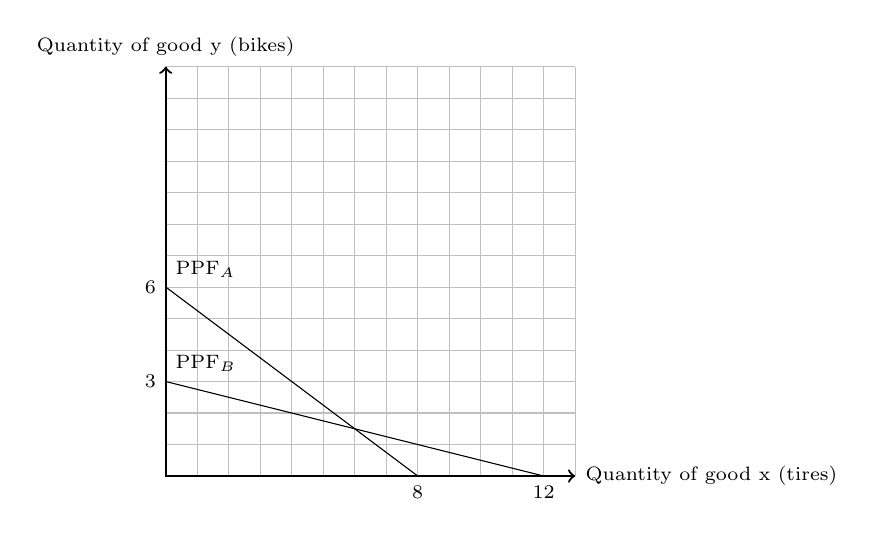
\begin{tikzpicture}[xscale=.4,yscale=.4]
				\draw [color=gray!50]  [step=10mm] (0,0) grid (13,13);
				\draw[thick,<->] (0,13) node[above,font=\scriptsize]{Quantity of good y (bikes)}--(0,0)--(13,0) node[right,font=\scriptsize]{Quantity of good x (tires)}; % 
				\draw (0,6) node[above right,font=\scriptsize] {PPF$_A$} -- (8,0) ;
				\draw (0,3) node[above right,font=\scriptsize] {PPF$_B$} -- (12,0) ;
				\node at (0,6)[left,font=\scriptsize]{6};
				\node at (0,3)[left,font=\scriptsize]{3};
				\node at (8,0)[below,font=\scriptsize]{8};
				\node at (12,0)[below,font=\scriptsize]{12};
				%			\draw[dotted] (0,0) -- (12,6);
				%	\draw[dotted] (0,0) -- (12,6);
				%	\node at (4,2)[circle,fill,inner sep=1.5pt]{};
				%	\node at (6,3)[circle,fill,inner sep=1.5pt]{};
				%	\draw[red] (0,6) -- (12,0);
			\end{tikzpicture}
		\end{center}	
		
		\abcx{
			\item How many \textbf{complete bikes}, i.e., one bike with two tires, can be consumed in autarky in country A and B, respectively. Draw the production points for country A and B into the figure. (A calculation is not necessary.)
			\item Calculate ---for both countries---the input coefficients, $a$, i.e., the units of labor needed to produce one unit of good $y$ and good $x$, respectively. Fill in the four input coefficients in the  following table:\bigskip
			
			\begin{center}\ttfamily
				\begin{tabular}{lcc}\toprule
					&\multicolumn{2}{c}{Countries}\\\cmidrule{2-3}
					&A &B\\		\midrule
					Good $y$ (bikes) & \rule{5em}{.4mm} & \rule{5em}{.4mm}\\
					Good $x$ (bike tires) & \rule{5em}{.4mm} & \rule{5em}{.4mm}\\\bottomrule
				\end{tabular}
			\end{center}\bigskip
			
			\item Fill in the ten gaps (\rule{5em}{.4mm}) in the following text:
			
			If we assume that both countries specialize completely in the production of the good at which they have a comparative advantage and trade is allowed and free of costs, then 
			\begin{itemize}
				\item
				country A produces \rule{5em}{.4mm} units of bikes and \rule{5em}{.4mm} units of tires and
				\item 
				country B produces \rule{5em}{.4mm} units of bikes and \rule{5em}{.4mm} units of tires.
			\end{itemize}
			Moreover, since both countries aim to consume complete bikes, i.e., one bike with two tires,
			\begin{itemize}
				\item
				country A exports \rule{4em}{.4mm} units of \rule{4em}{.4mm} and imports \rule{4em}{.4mm} units of \rule{4em}{.4mm} and 
				\item 
				country B exports \rule{4em}{.4mm} units of \rule{4em}{.4mm} and imports \rule{4em}{.4mm} units of \rule{4em}{.4mm}.
			\end{itemize}
			Under free trade 
			\begin{itemize}
				\item country A can consume \rule{5em}{.4mm} complete bikes and 
				\item country B can consume \rule{5em}{.4mm} complete bikes.
			\end{itemize}
			
	}}
	
	\pbn
	\solx{Bikes and bike tires}{
		\abcx{
			\item 		Both countries can consume 2 complete bikes. 
			\begin{center}
				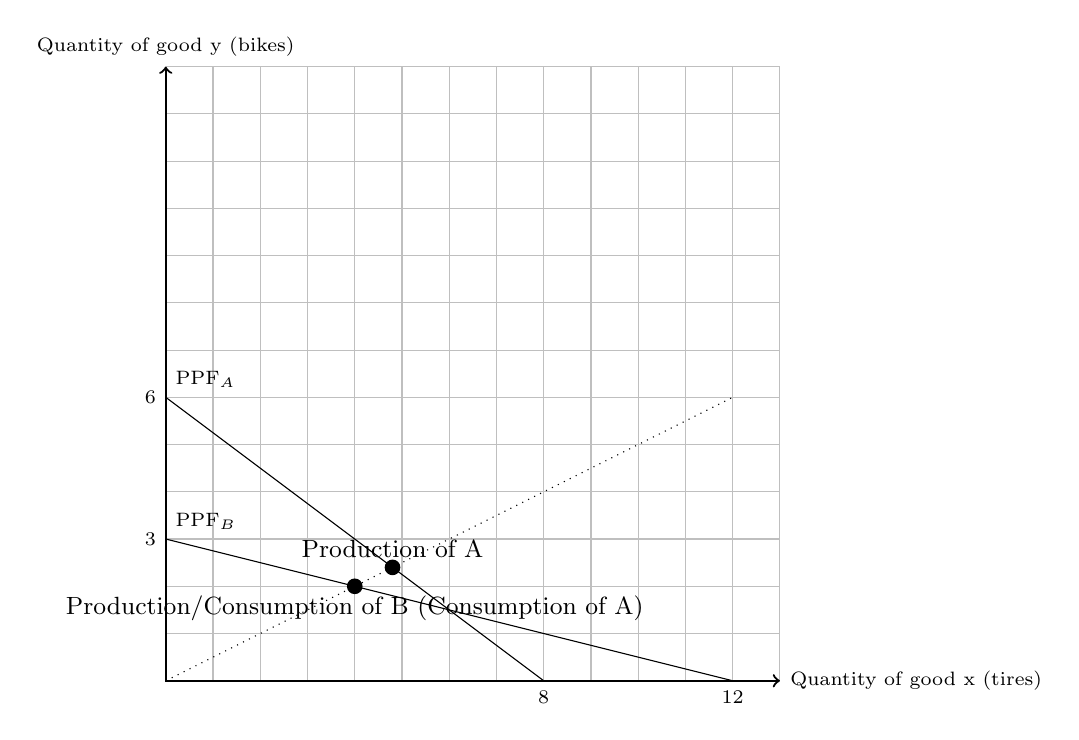
\begin{tikzpicture}[xscale=.6,yscale=.6]
					\draw [color=gray!50]  [step=10mm] (0,0) grid (13,13);
					\draw[thick,<->] (0,13) node[above,font=\scriptsize]{Quantity of good y (bikes)}--(0,0)--(13,0) node[right,font=\scriptsize]{Quantity of good x (tires)}; % 
					\draw (0,6) node[above right,font=\scriptsize] {PPF$_A$} -- (8,0) ;
					\draw (0,3) node[above right,font=\scriptsize] {PPF$_B$} -- (12,0) ;
					\node at (0,6)[left,font=\scriptsize]{6};
					\node at (0,3)[left,font=\scriptsize]{3};
					\node at (8,0)[below,font=\scriptsize]{8};
					\node at (12,0)[below,font=\scriptsize]{12};
					\draw[dotted] (0,0) -- (12,6);
					%	\draw[dotted] (0,0) -- (12,6);
					\node at (4,2)[circle,fill,inner sep=2pt]{};
					\node at (4,2)[below,font=\small]{Production/Consumption of B (Consumption of A)};
					\node at (48/10,48/20)[circle,fill,inner sep=2pt]{};
					\node at (48/10,48/20)[above,font=\small]{Production of A};
					%			\node at (12,0)[below,font=\scriptsize]{12};
					%	\node at (6,3)[circle,fill,inner sep=1.5pt]{};
					%	\draw[red] (0,6) -- (12,0);
				\end{tikzpicture}
			\end{center}\bigskip
			\item The table\\
			\begin{center}
				\begin{tabular}{lcc}\toprule
					input	&\multicolumn{2}{c}{Countries}\\\cmidrule{2-3}
					cooeficients	&A &B\\		\midrule
					Good $y$ (bikes) & 24:6=4 &24:3=8\\
					Good $x$ (bike tires) & 24:8=3 &24:12=2 \\\bottomrule
				\end{tabular}
			\end{center}\bigskip
			
			\item
			If we assume that both countries specialize completely in the production of the good at which they have a comparative advantage and trade is allowed and free of costs, then 
			\begin{itemize}
				\item
				country A produces 6 units of bikes and 0 units of tires and
				\item 
				country B produces 0 units of bikes and 12 units of tires.
			\end{itemize}
			Moreover, since both countries aim to consume complete bikes, i.e., one bike with two tires,
			\begin{itemize}
				\item
				country A exports 3 units of bikes  and imports 6 units of tires  and 
				\item 
				country B exports 6 units of tires and imports 3 units of bikes.
			\end{itemize}
			Under free trade 
			\begin{itemize}
				\item country A can consume 3 complete bikes and 
				\item country B can consume 3 complete bikes.
			\end{itemize}
			
	}}
	
		\pbn
	\exextoc{Ricardian model MC}{
		Assume that only two countries, A and B, exist. Both countries are equally endowed with the only production factor labor which can be used to produce either good $y$ or good $x$. The table below gives input coefficients, $a$, for both countries, i.e., the units of labor needed to produce one unit of good $y$ and good $x$, respectively.
		\begin{center}
			\begin{tabular}{lcc}\toprule
				&\multicolumn{2}{c}{Countries}\\\cmidrule{2-3}
				&A &B\\		\midrule
				Good $y$ & 321 & 899\\
				Good $x$ & 459 & 999 \\\bottomrule
			\end{tabular}
		\end{center}
		Which of the following statements is true? 
		\begin{enumerate}[a)]
			\item  Country A has an absolute advantage in both goods.
			\item  Country A has an absolute advantage in good $y$ 
			\item  Country A has a comparative advantage in both goods.
			\item  Country B has a comparative advantage in both goods.
			\item  Country A has a comparative advantage in good $y$.
			\item  Country B has a comparative advantage in good $y$.
		\end{enumerate}
	}
	
	\pbn
	\solx{Ricardian model MC}{a), b), and e) are correct statements.}	
	

	
	
	
	%
	
	\section{Trade because of different endowments (Heckscher-Ohlin model)}\label{sec:ho}
	
	%\begin{shadedbox}
	%	Please watch the video available on ILIAS, see: 
	%	
	%	\url{Heckscher Ohlin Lecture Part A}
	%	
	%and
	%
	%\url{Heckscher Ohlin Lecture Part B}
	%\end{shadedbox}	
	
	
	
	\subsection{Nobel prize winning theory}
	The Model which we discuss in this section is named after two Swedish economist, Eli Heckscher (1879-1952) and Bertil Ohlin (1899-1979). Bertil Ohlin received the Nobel Prize in 1977 (together with James Meade). The HO-Model, as it is often abbreviated, was the main reason for the price. 
	Here is an excerpt of the Award ceremony speech:
	\boxb{
		\begin{quotation}
			Your Majesties, Your Royal Highnesses, Ladies and Gentlemen,
			
			The question why individuals, firms and nations exchange goods and services with each other, and how these processes are influenced by government policies, may be regarded as the basic issue in the science of economics. In the case of exchange between countries, the dominating theory was for a long time – from the beginning of the 19th century – David Ricardo’s theory of comparative advantage. Ricardo explained there the structure of foreign trade by differences in the production technology between nations. Over the years the theory was gradually improved upon in various ways, but a more basic overhaul did not take place until Bertil Ohlin in the early 1930’s published his work Interregional and International Trade, which is now a classic, and James Meade in the 1950’s came out with his important volumes on The Theory of International Economic Policy.
			
			Bertil Ohlin showed in this work, which to some extent was inspired by a remarkable article by Eli Heckscher, that foreign trade may arise even if the production technology were identical in different nations. It is enough that the supplies of the factors of production of various kinds – such as labor of different types, capital, and land – differ among nations. The starting point of Ohlin’s theory is that a country tends to be an exporter of commodities that use relatively large amounts of the factors of production which are in ample supply as compared to domestic demand – in the hypothetical case without foreign trade. For instance, to take a simple example, if land is abundant in Australia while labor is relatively plentiful in England, we would expect Australia to be an exporter of commodities which for their production require much land, such as wool, while England would be an exporter of commodities the production of which requires relatively much labor, such as textiles.
			
			From this simple theoretical structure, the so-called Heckscher-Ohlin model, follow a number of interesting theorems. One of them, the factor price equalization theorem, tells us that foreign trade tends to equalize the prices of the factors of production in different countries. For instance, when Australia starts to export land-intensive goods, the demand for land goes up relative to labor, with a rise in land prices as a result, while the export of labor-intensive goods by England pulls up wages there relative to the price of land. Thus, trade in commodities tends to have the same effects on the prices of the factors of production as if the factors themselves could move freely between countries. In this sense, commodity trade is a substitute for international mobility of the factors of production. Another inference from Ohlin’s theory is that a tariff on a labor-intensive good, such as textiles, affects the distribution of income in favor of labor in the importing country, while a tariff on a capital-intensive commodity, such as wool or steel, results in an income redistribution in favor of the owner of capital.
			
			Source: \url{https://www.nobelprize.org/prizes/economic-sciences/1977/ceremony-speech}
		\end{quotation}
	}
	
	The Ricardo model explains international trade as advantageous because of comparative advantages that are the result of technological differences. This means that comparative advantage in the Ricardian model is solely the result of \textbf{productivity differences}. The size of a country or the size of the countries' endowments does not matter for comparative advantage in the Ricardian model because there is only one factor of production in Ricardian models, namely labor. However, the assumption that there is only one factor of production is unrealistic, and we should ask what happens \textbf{if there is more than one factor of production but no productivity differences}? 
	What happens if the two factors are available differently in different countries? What is the significance of endowment differences for international trade? And which owner of a factor of production will be a winner when a country opens up to world trade, and who will lose? The HO model can provide answers to these questions. 
	
	In \autoref{tab:endow}, I show that countries do indeed differ substantially in their total factor productivity, capital stock, and labor endowments, which are likely correlated with total population. 
	
	\pbn
	\subsection{The Heckscher-Ohlin (factor proportions) model}
	Assumptions:
	\enux{
		\item \textbf{Two countries}: Home country and foreign country. Variables referring to foreign countries are marked with an asterisk, $*$.
		\item \textbf{Two goods}: $x$ and $y$.
		\item \textbf{Two factors of production}: $K$ and $L$.
		This is new in relation to the Ricarkian model! Let's name the factors $K$ and $L$, which stands for capital and labor. 
		\item \textbf{Goods differ in terms of their need for factors of production}: $\frac{K_y}{L_y} \neq \frac{K_x}{L_x}.$\\
		This means that one good must be produced in a capital-intensive way and the other in a labor-intensive way. If we assume that good $y$ is capital intensive and good $x$ is labor intensive in production, we can write:
		\begin{align*}
			\frac{K_y}{L_y} > \frac{K_x}{L_x}.
		\end{align*}
		In this inequality, the quantity of capital required to produce good $y$, $K_y$, is on the left-hand side relative to the quantity of labor required to produce good $y$, $L_y$, i.e., the capital intensity of good $y$.The capital intensity of good $x$ is on the right-hand side of the inequality.  Rewriting this inequality, we can express it in terms of labor intensities:
		$\frac{L_y}{K_y} < \frac{L_x}{K_x}.$
		It should be clear that both inequalities say the same thing. 
		\item \textbf{No technology differences between countries}:\.
		Since we already know from Ricardian theory that productivity or technology differences are a source of international trade, we do not want to explain the same thing again with the HO model.  So we assume that all input coefficients are the same in all countries. 
		\item \textbf{Different relative factor endowments}: $\frac{K}{L} \neq \frac{K^*}{L^*}$\\
		Since countries are assumed to have different factor endowments, the model links a country's trade pattern to its endowment of factors of production. The capital-labor ratio in the home country, $\frac{K}{L}$, must differ from the ratio abroad.
		Suppose the home country is capital-rich and the foreign country is labor-rich. Then we have the following ratios between capital and labor in the two countries:
		\begin{align*}
			\frac{K}{L} > \frac{K^*}{L^*}.
		\end{align*}
		This means that the capital-labor ratio (a country's capital intensity) is higher in the home country than abroad.
		In terms of the ratio between labor and capital, i.e., the labor intensity of a country, this can be expressed as follows:
		$\frac{L}{K} < \frac{L^*}{K^*}.$
		It should be clear that both inequalities say the same thing. 
		
		\item \textbf{Free factor movement between sectors}
		Both factors can be used in the production of both goods. Note that cross-country movement of factors (migration, foreign direct investment) is not allowed.
		\item \textbf{No trade costs}
		Final products can be traded without any costs.
		\item \textbf{Equal tastes in countries and homothetic preferences}
		Consumers in both countries have the same utility function. Homothetic preferences simply mean that for given relative prices, income does not affect the ratio of consumption.
	}
	
	\pbn
	\subsection{Intuition}
	\itex{
		\item Consider that the home country has relatively more capital and the foreign country relatively more labor and that the good $y$ is capital intensive in production whereas the good $x$ is labor intensive. 
		\item Then it is relatively cheap for the home country to produce the capital-intensive good because it is endowed with a lot of capital, while it is relatively costly to produce the good with which the country is hardly endowed. 	
		\item Thus, the home country has a comparative advantage in producing the capital-intensive good.
		\item The opposite is true for the foreign country.
	}
	
	\heux{Heckscher-Ohlin Theorem}{
		The capital abundant country exports the capital-intensive good.
		The labor abundant country exports the labor-intensive good.\\
		Or:\\
		A country export goods that are intensive in its relatively abundant factor and will import goods that are intensive in its relatively scarce factor.
	}\medskip
	
	\itex{
		
		\item As a result of the Heckscher-Ohlin theorem, output of the good in which the country has a comparative advantage would increase. The capital intensive country will produce more capital intensive goods and the labor intensive country will produce more labor intensive goods.
		\item As the production of the good that makes intensive use of the abundant resource increases, the demand for that resource will also increase. Demand for the scarce resource will also increase, but to a lesser extent.
		\item If production of the good that intensively uses the scarce resource decreases, both abundant and scarce resources will be released, but relatively more of the scarce resource than of the abundant resource.
		\item In autarky, the relatively scarce factor in the home country was labor and factor prices were as follows:
		\[
		\frac{w}{r}>\frac{w^*}{r^*}
		\] 
		\item After opening to trade, production shifts to the home country so that the wage falls ($w\downarrow$) and the rent rises ($r\uparrow$).
		\item After opening to trade, production shifts abroad so that the wage rises, $w^*\uparrow$, and the rent falls, $w^*\downarrow$.
		\item This reallocation process, and hence the change in factor prices, continues until factor prices are equal in all countries:
		\[
		\frac{w}{r}=\frac{w^*}{r^*}
		\] 	
		\item \autoref{fig:hofactor} visualizes this line of reasoning. 
		\item I recommend a clip of Mike Moore explaining how trade based on factor endowments affects wages and returns to capital, see \tv \url{https://youtu.be/qk4tdP6ta78}
	}
	
	\begin{centering}
		\begin{tikzpicture}[xscale=.8,yscale=.8]
			%	\draw [color=gray!50]  [step=10mm] (0,0) grid (10,10);
			\draw[thick,<->] (0,10) node[left]{$\frac{p_y}{p_x}$}--(0,0)--(10,0) node[right]{$\frac{w}{r}$}; 
			\coordinate  (yH) at (1,9);
			\coordinate (xH) at (9,1);
			\coordinate (F) at (7,3);
			\coordinate (H) at (3,7);
			\coordinate (Fx) at (7,0);
			\coordinate (Hx) at (0,7);
			\coordinate (WW) at (5,5);
			\draw[dashed] (Fx) node[below] {$\left(\frac{w}{r}\right)^H_{\textnormal{autarky}}$} -- (F) -- (0,3) node[left] {$\left(\frac{p_y}{p_x}\right)^H_{\textnormal{autarky}}$};
			
			\draw[dashed] (Hx) node[left] {$\left(\frac{p_y}{p_x}\right)^F_{\textnormal{autarky}}$} -- (H) -- (3,0) node[below] {$\left(\frac{w}{r}\right)^F_{\textnormal{autarky}}$};	
			
			\draw[dashed] (0,5) node[left] {$\left(\frac{p_y}{p_x}\right)^*_{\textnormal{free trade}}$} -- (WW) -- (5,0) node[below] {$\left(\frac{w}{r}\right)^*_{\textnormal{free trade}}$};
			
			\draw (xH) -- (yH) node[above right] {};
			\foreach \n in {F, H, WW}
			\node at (\n)[circle,fill,inner sep=1.5pt]{};
			\draw[-{Latex[length=3mm]}] (7,1) -- (5,1);
			\draw[-{Latex[length=3mm]}] (3,1) -- (5,1);
			\draw[{Latex[length=3mm]}-] (1,5) -- (1,7);
			\draw[{Latex[length=3mm]}-] (1,5) -- (1,3);	
		\end{tikzpicture}
		\captionof{figure}{HO Model and factor prices}\label{fig:hofactor}\end{centering}	
	
	
	
	\heux{Factor-Price Equalization Theorem}{The prices of the two factors of production (wage and rent) will be equalized across countries as a result of international trade in goods.}
	
	
	
	\subsubsection{Why does the Factor-Price Equalization Theorem not (fully) hold?}
	In the real world, factor prices do not equalize due to frictions such as transportation costs, trade barriers, and the presence of goods that are rarely or never traded.
	
	\subsubsection{Trade as an alternative to factor movements }
	The factor price equalization theorem contains an interesting insight: if a country allows free trade in its products, it will automatically export the abundant factor indirectly in the form of goods that intensively use the abundant factor.
	%In recent years countries such as Ireland, the Philippines, India, Jamaica, and Bangladesh, China, and Malaysia have been doing just that.
	
	\pbn
	\exextoc{Ricardo and Heckscher-Ohlin}{	
		\abcx{
			\item Discuss the main differences of the Ricardian Model and the Heckscher-Ohlin Model. 
			\item Assume that only two countries, A and B, exist. Both countries are equally endowed with the only production factor labor which can be used to produce either good $y$ or good $x$. The table below gives input coefficients, $a$, for both countries, i.e., the units of labor needed to produce one unit of good $y$ and good $x$, respectively.\label{error:mis} \medskip
			\begin{center}
				\begin{tabular}{lcc}\toprule
					&\multicolumn{2}{c}{Countries}\\\cmidrule{2-3}
					&A &B\\		\midrule
					Good $y$ & 10 & 11 \\
					Good $x$ & 1 & 2 \\\bottomrule
				\end{tabular}
			\end{center}\medskip
%			\begin{enumerate}[i)]
%				\item Name the country with an absolute advantage.
%				\item 
				Name the country with a comparative advantage in good $y$.
%			\end{enumerate}
	}}
	
	
	\pbn
	\exextoc{HO-Model in one figure}{
		Suppose consumers from country A and the foreign country B like to consume two goods that are neither perfect substitutes nor perfect complements. Moreover, assume for simplicity that both countries have the same size but have different endowments, as stated in the assumptions above. 
		Moreover, assume the factor intensity of production as stated in the assumptions above.\label{error:hopic}
		\abcx{
			\item Sketch the production frontiers for both countries in autarky. Show graphically the relative price in autarky.
			\item You will see that the relative prices of goods differ across countries:
			\begin{align*}
				\left(\frac{p_1}{p_2}\right)\neq\left(\frac{p_1}{p_2}\right)^*.
			\end{align*}
			That means, the Home country A has a comparative advantage in producing good $1$. 
			\item Now, sketch the world market price that will maximize the utility. 
			\item Where are the new production and consumption points of both countries?
			\item Show in the graphic how much each country trades.
			\item I recommend a clip of Mike Moore who also explains the HO-Model with production possibility curves, see \tv	\url{https://youtu.be/F_CfnAbytxk} 
	}}
	
	\solx{HO-Model in one figure}{\bigskip \begin{center}
			\includegraphics[width=.5\linewidth]{../../../pic/hoexa2}\label{fig:hoexa}	\captionof{figure}{HO-Model in one figure}
			\note{Source: Own drawing based on  \cite{Wikipedia2020Trade}.}
		\end{center}
		Two identical countries (A and B) have different initial factor endowments. I assume that country A	 is abundantly endowed with the production factor that is intensively used in the production of good 1, the reverse holds for country B.
		Thus, the two solid black lines in \autoref{fig:hoexa} represents the respective production possibility frontier curves. The orange lines represents the respective indifference curves. Autarky equilibria are marked with $A^{A}$ and $A^{B}$, respectively. The production points in trade equilibrium are marked with $P^A$ and $P^B$, the consumption point of both countries is in $C^A=C^B$. Thus, production and consumption points are divergent. The indifference curve under free trade is clearly above the other indifference curve in autarky. The solid black line that is tangient to the consumption point under free trade represents the utility maximizing world market price under free trade. The exports, $X$, and imports; $I$, are denotes correspondingly to the goods and country names. 
	}
	
	\pbn
	 \exextoc{Multiple choice: HO-Model}{Given are the assumptions of the Heckscher-Ohlin Model. In particular, assume that only two countries, A and B, and two goods, $y$ and $x$, exist. Consider the following data:\label{error:addho}
	\begin{center}
		\begin{tabular}{lcc}\toprule
			&\multicolumn{2}{c}{Countries}\\\cmidrule{2-3}
			Factor Endowments & A &B\\		\midrule
			Labor Force & 20 & 30\\
			Capital Stock & 30 & 40 \\\bottomrule
		\end{tabular}
	\end{center}
	If good $y$ is capital intensive in production and good $x$ is labor intensive in production then, following the Heckscher-Ohlin Theorem, \dots
	\abcx{
		\item \dots country A will export good $y$.
		\item \dots country B will export good $y$.
		\item \dots both countries will export good $y$.
		\item \dots trade will not occur between these two countries.
	}
}

\pbn
\solx{Multiple choice: HO-Model}{
Answer a) is correct.	
}
	
	%\input{../stata/endow}
	\begin{table}[H] \centering%
		\caption{Endowment differences across countries in 2010}%
		{\tiny
			\begin{tabularx}{\textwidth}{lCCC}
				\toprule
				&(1)&(2)&(3) \tabularnewline
				RegionCode&Capital stock at current PPPs (in mil. 2011USD)&Population (in millions)&Capital stock per capita \tabularnewline
				\midrule\addlinespace[1.5ex]
				ITA&10421041&60&174885 \tabularnewline
				ESP&7806612&47&167518 \tabularnewline
				FRA&10405968&65&160395 \tabularnewline
				GBR&9973122&63&159019 \tabularnewline
				DEU&12687682&80&157738 \tabularnewline
				USA&48876336&310&157729 \tabularnewline
				AUS&3332890&22&150382 \tabularnewline
				CAN&5065392&34&148431 \tabularnewline
				JPN&17161376&127&134790 \tabularnewline
				SAU&3716382&28&132300 \tabularnewline
				KOR&6052155&49&123287 \tabularnewline
				TWN&2835890&23&122549 \tabularnewline
				ROU&1271652&20&62647 \tabularnewline
				VEN&1765996&29&60905 \tabularnewline
				BRA&9869311&199&49691 \tabularnewline
				RUS&6746460&143&47126 \tabularnewline
				POL&1769004&39&45859 \tabularnewline
				THA&2977965&67&44652 \tabularnewline
				IRN&3234132&74&43555 \tabularnewline
				ARG&1773984&41&43034 \tabularnewline
				MEX&5054693&119&42613 \tabularnewline
				TUR&2938288&72&40634 \tabularnewline
				UKR&1616826&46&35420 \tabularnewline
				IDN&8146254&242&33716 \tabularnewline
				COL&1446480&46&31501 \tabularnewline
				CHN&42218080&1341&31483 \tabularnewline
				PER&681036&29&23185 \tabularnewline
				PHL&1560017&93&16767 \tabularnewline
				IRQ&443733&31&14375 \tabularnewline
				IND&15356803&1231&12475 \tabularnewline
				\bottomrule \addlinespace[1.5ex]
				\multicolumn{4}{p{\textwidth}}{\begin{footnotesize} Source: Penn World Tables 9.0\end{footnotesize}}
			\end{tabularx}%
		}
		\label{tab:endow}%
	\end{table}%
	
	
	\pbn
	\section{The specific factor model}\label{sec:specific}
	
	\begin{center}
		\includegraphics[width=.6\linewidth]{$HOME/Dropbox/hsf/pic/ie/freetradeatlast_pdf}
%		\captionof{figure}{Free trade at last}\label{fig:freetradeatlast2}
\note{Source: \url{https://otherwords.org/wp-content/uploads/2015/03/Free-trade-at-last.jpg}}
%\bigskip
	\end{center}
	
	\pbn
	From the Ricardian model, we know that trade is a positive-sum game. 
	If free trade is beneficial to a country, as Ricardo predicts, why isn't everyone happy with free trade? 
	In democratic societies, policymakers sometimes adopt protectionist trade policies because of pressure from interest groups and public demand. 
	The discrepancy between the promises and potential benefits of trade on the one hand and the negative consequences of free trade for many groups on the other is illustrated in \autoref{fig:freetradeatlast} \textit{Free trade at last}. The models so far do not give us a way to see which groups actually suffer from free trade, and thus we have no clue  why there are incentives for interest groups to oppose free trade. 
	Are anti-free trade policy preferences the result of ignorance, general worldviews, political ideology, environmental attitudes, social trust, or other factors? Well, these things may play a role, but there are also economic factors, i.e., the self-interest of individuals and groups within an economy, that can account for anti-free trade attitudes.
	In the following sections, we will discuss a theory that shows that while free trade benefits countries as a whole, not everyone within a country benefits equally. Some benefit more than others, and some are actually made worse off by free trade. 
	
	In the next two subsections, we derive some key hypotheses that free trade favors those people in a country who have abundant factors of production and disadvantages those who have scarce factors. Moreover, free trade favors investors and workers in export-oriented industries with comparative advantages.
	
	\pbn
	\subsubsection{Assumptions}
	The sector-specific model, also known as the Ricard-Viner model, can show that there are winners and losers in international trade. The model is based on the following assumptions:
	\enux{
		\item 2 countries $i \in \{A, B\}$
		\item 2 goods (sectors) $g \in \{1, 2\}$
		\item 3 factors of production: Labor $L$, capital specific to the production of good 1, $K_1$, and capital specific to the production of good 2, $K_2$\footnote{You can think of capital specific to the production of manufacturing goods (good 1) and land specific to the production of food sector goods (good 2)}.
		\ The technologies for the production of both goods are now represented by two
		production functions $Q_1=F_1(\bar{K_1},L_1)$ and $Q_2=F_2(\bar{K_2},L_2)$, where both factors of production have positive but decreasing marginal products
		\item The capital allocated to each sector is fixed for both countries: $K_1=\bar{K}_{1}, K_2=\bar{K}_{2}$
		\item The labor assigned to each sector ($L_1$ and $L_2$) can change in response to
		Response to external shocks: $\bar{L}=L_1+L_2$
		\item perfect competition
		\item perfect market clearing (no unemployment)
		\item country A is a small open economy (we consider only country A and therefore do not use a subscript for countries in the following)
	}\bigskip
	
	
	\begin{minipage}{0.4\linewidth}	
		\paragraph{The production possibility frontier with two factor inputs:}
		The two production functions, the fixed endowments and the distribution of labor determine the aggregate PPF. The PPF, which is the product of two production functions ($F_1$ and $F_2$), is shown in \autoref{fig:ppftwo}. The figure shows, for both production points A and B, how the mobile factor of production, labor, must be reallocated from sector 2 to sector 1 in order to produce more of good 1 in production point B. The second and fourth quadrants show the respective production functions of sectors 1 and 2.
	\end{minipage}
	\begin{minipage}{0.6\linewidth}	
		\begin{centering}
			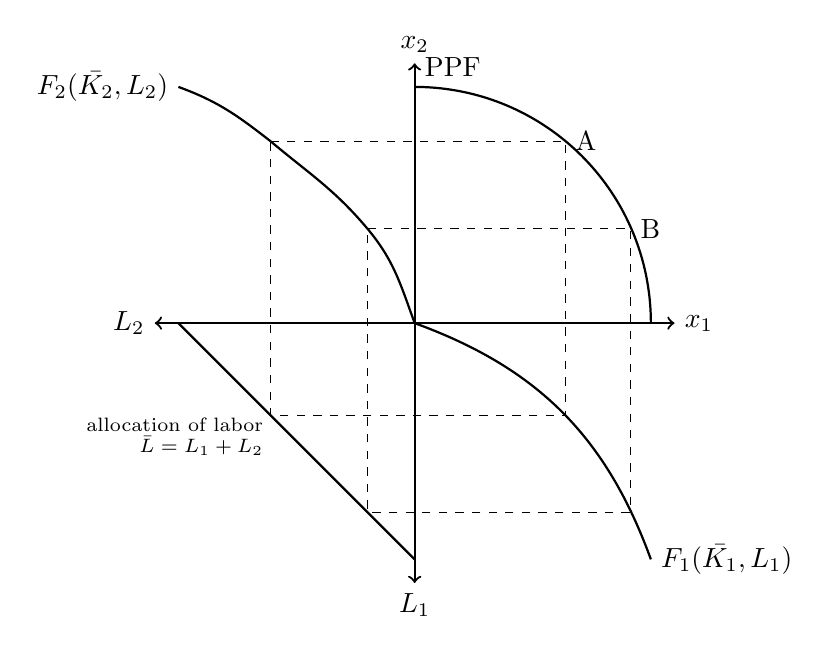
\begin{tikzpicture}[xscale=.3,yscale=.3]
				%	\draw [color=gray!50]  [step=5mm] (-11,-11) grid (11,11);
				\draw[thick,<->] (0,11) node[above]{$x_2$}--(0,0)--(11,0) node[right]{$x_1$}; 
				\draw[thick,<->] (0,-11) node[below]{$L_1$}--(0,0)--(-11,0) node[left]{$L_2$}; 
				
				\coordinate (lmx) at (0,-10);
				\coordinate (lmy) at (-10,0);
				\draw[thick] (lmx) -- (lmy);
				\node[above left,font=\scriptsize] (name) at (-6,-5) {allocation of labor};
				\node[above left,font=\scriptsize] (name) at (-6,-6) {$\bar{L}=L_1+L_2$};
				
				\draw[thick] (0,0) to [out=110,in=-50] (-2,4) ;
				\draw[thick] (-2,4) to [out=130,in=-40] (-6.1,7.7) ;
				\draw[thick] (-6.1,7.7) to [out=142,in=-20] (-10,10)  node[left] {$F_2(\bar{K_2},L_2)$};	
				
				\draw[thick] (0,0) to [out=-20,in=110] (10,-10) node[right] {$F_1(\bar{K_1},L_1)$};
				\draw[thick] (10,0) to [out=90,in=0] (0,10) node[above right] {PPF};
				
				\draw [dashed] (-2,4) -- (9.15,4) node[right] {B} -- (9.15,-8)  -- (-2,-8) -- (-2,4)  ;
				\draw[dashed]  (-6.1,7.7) -- (6.4,7.7) node[right] {A} -- (6.4,-3.9) -- (-6.1,-3.9) -- (-6.1,7.7)  ;
			\end{tikzpicture}
			\captionof{figure}{PPF with two factors and positive but declining marginal products}\label{fig:ppftwo}\end{centering}\bigskip
	\end{minipage}
	
	\pbn
	\paragraph{Equillibrium in autarky:}
	\itex{
		\item Depending on a country's demand for good 1 and 2 a production point on the PPF is chosen at which it must hold that the slope of the PPF curve and the price relation (i.e., relation of marginal product of labor in sector 1 and sector 2) must be equal:
		\begin{align*}
			\frac{p_1}{p_2}=\frac{\frac{\partial F_2}{\partial L_2}}{\frac{\partial F_1}{\partial L_1}}
		\end{align*}
		\item What can we say about the rents of the production factors?
		\item From the assumption of perfect competition it follows that firms do not make a positive profit in equilibrium, $\pi\overset{!}{=}0$. Thus, the equilibrium wage for sectors $g \in \{1, 2\}$ are given by the profit maximizing of firms
		\begin{align*}
			\pi_g&=p_g\cdot F_g(\bar{K_g},L_g)-w_gL_g-r_gK_g\\
			\frac{\partial \pi_g}{\partial L_g}&= p_g\cdot \frac{\partial F_g}{\partial L_g}-w_g\overset{!}{=}0 \qquad
			\Leftrightarrow w_g=p_g\frac{\partial F_g}{\partial L_g}
		\end{align*}
		\item We know that labor can move freely between sectors and an equilibrium exists when there are no incentives to move any further. That is the case when wages in both sectors are equal, $w_1=w_2$. 
		Thus, we can express wages in terms of purchasing power in units of good 1 as follows: 
		\begin{align*}
			w_1&=p_1\frac{\partial F_1}{\partial L_1}\qquad \textnormal{ and } \qquad w_2=p_2\frac{\partial F_2}{\partial L_2}\\
			\Rightarrow w&=p_1\frac{\partial F_1}{\partial L_1}=p_2\frac{\partial F_2}{\partial L_2}\\
			\Leftrightarrow \frac{w}{p_1}&=\frac{\partial F_1}{\partial L_1}\\
			\Leftrightarrow \frac{w}{p_2}&=\frac{\partial F_2}{\partial L_2}
		\end{align*}
		\item \autoref{fig:eqaut} presents the equilibrium wage and the optimal allocation of labor into sector 1 and 2.
	}\bigskip
	
	\begin{centering}
		\begin{tikzpicture}[xscale=.9,yscale=.6]
			\draw[thick,<->] (0,12) node[above]{$w$}--(0,0) node[below] {$L_1=0$} --(11,0) node[right]{$L_1$};
			\draw[thick,<->] (-1,0) node[left]{$L_2$}  -- (10,0) node[below] {$L_2=0$} --(10,12) node[above]{$w$};
			
			\draw (0.2,3) to[out=0,in=-100] (9.8,10.8) node[left]{$p_2\cdot\frac{\partial f}{\partial L_2}$};
			\draw (0.2,9.8) node[right]{$p_1\cdot\frac{\partial f}{\partial L_1}$} to[out=-80,in=-180] (9.8,1);
			
			\coordinate (eqA) at (3.45,3.46);
			\node[above] at (eqA) {A};
			\foreach \n in {eqA}
			\node at (\n)[circle,fill,inner sep=1.5pt]{};
			
			\draw[dotted]  (0,3.46) node[left] {$w$} -- (10,3.46)  node[right] {$w$};
			\draw[dotted] (eqA) -- (3.46,0);
			%\draw[dotted] (0,3.46) -- (6.13,3.46);
			
			\draw [thick,decoration={brace,mirror,amplitude=10pt,raise=-5pt},decorate] (0,-1.4) -- (3.45,-1.4) node[midway,below,yshift=-.1cm] {$L_1$};
			\draw [thick,decoration={brace,mirror,amplitude=10pt,raise=-5pt},decorate] (3.45,-1.4) -- (10,-1.4) node[midway,below,yshift=-.1cm] {$L_2$};
			\draw [thick,decoration={brace,mirror,amplitude=10pt,raise=-5pt},decorate] (0,-3) -- (10,-3) node[midway,below,yshift=-.3cm] {$L$};
		\end{tikzpicture}
		\captionof{figure}{Equilibrium in autarky}\label{fig:eqaut}\end{centering}\bigskip
	
	\pbn
	\paragraph{Equilibrium under free trade:}
	Assume the price of good 1 and good 2 increase due to a trade opening in the same proportion. What happens with the real wage and the real incomes of capital-1 and capital-2 owners? The answer is: no real changes occur. 
	\itex{\item The wage rate, $w$, rises in the same proportion as the prices, so the real wages are unaffected. In \autoref{fig:ppftwo} this can be shown by shifting both curves upward.
		\item The real incomes of capital owners also remain the same because there will be no reallocation of labor across sectors.}
	Now, assume only the price of good 1 rises for 10\% while $p_2$ remains fixed, $\frac{p'_1}{p_2}>\frac{p_1}{p_2}$.  What happens with the real wage and the real incomes of capital-1 and capital-2 owners? The answer is: some win, some lose, and some maybe win.
	
	\textbf{Wages:}
	\itex{
		\item $p_1\frac{\partial F_1}{\partial L_1}$ rises and hence labor reallocates from sector 2 to sector 1 ($L_1\uparrow$ and $L_2\downarrow$). This is shown in \autoref{fig:eqfree}.
		\item This reallocation of labor has some implications for the real wages measured in purchasing power of good 1 and 2, respectively:
		\item The price of good 1 has increased by 10\%, the wage has however increased by less than 10\% (compare the length of BC and BD in the figure), whereas the price for food stays constant. 
		\item  Thus, the purchasing power in buying good 2 increased, whereas the purchasing power in buying good 1 decreased. Hence, workers gain when buying good 2 but lose when buying good 1
		\item Overall, the welfare effect from real wages is unclear and depends on preferences.
	}
	\textbf{Owner of capital-1:}
	\itex{\item Owners of capital-1 receive a 10\% higher price on their products but have to pay a less than 10\% higher wage.
		\item Overall, capital-1 owners gain from free trade because they can employ more workers (at a higher price) now.
	}
	\textbf{Owner of capital-2:}
	\itex{\item Owner of capital-2 receive the same price on their products but have to pay a higher wage.
		\item Overall, capital-2 owners lose from free trade because they can employ less workers at a higher price now.
	}
	
	
	\begin{centering}
		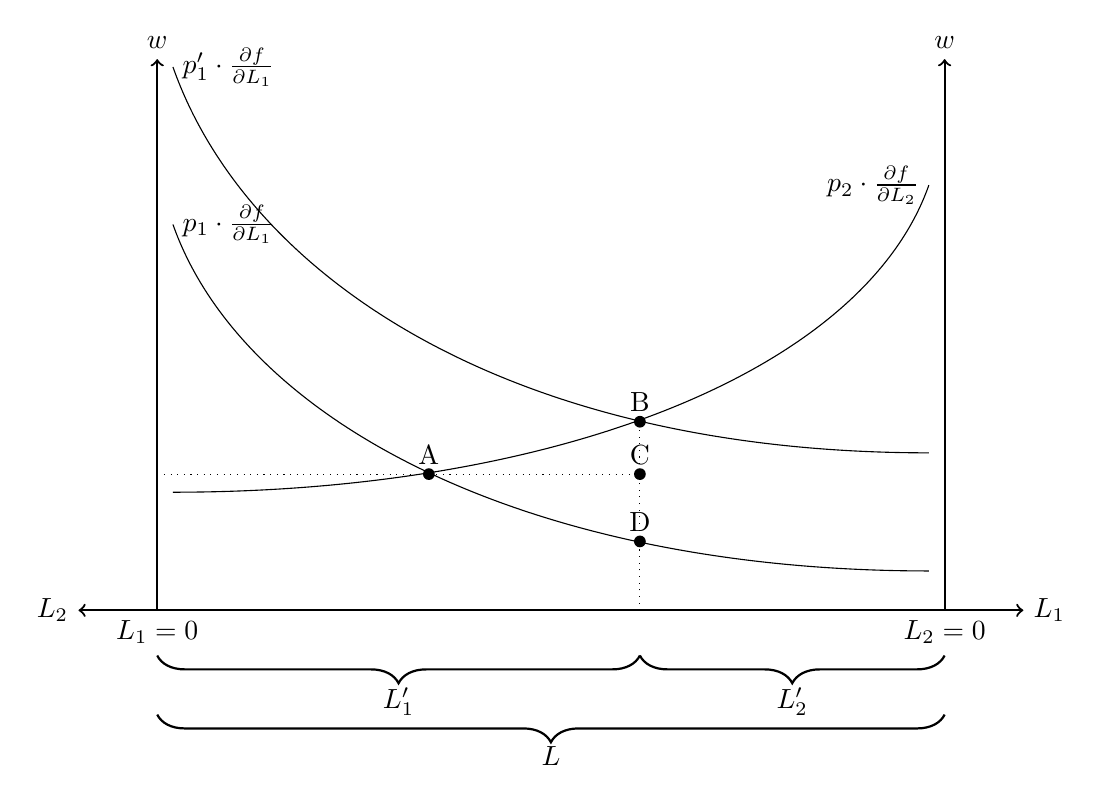
\begin{tikzpicture}[xscale=1,yscale=.5]
			\draw[thick,<->] (0,14) node[above]{$w$}--(0,0) node[below] {$L_1=0$} --(11,0) node[right]{$L_1$};
			\draw[thick,<->] (-1,0) node[left]{$L_2$}  -- (10,0) node[below] {$L_2=0$} --(10,14) node[above]{$w$};
			
			\draw (0.2,3) to[out=0,in=-100] (9.8,10.8) node[left]{$p_2\cdot\frac{\partial f}{\partial L_2}$};
			\draw (0.2,9.8) node[right]{$p_1\cdot\frac{\partial f}{\partial L_1}$} to[out=-80,in=-180] (9.8,1);
			\draw (0.2,13.8) node[right]{$p'_1\cdot\frac{\partial f}{\partial L_1}$} to[out=-80,in=-180] (9.8,4);
			\coordinate (eqB) at (6.13,4.79);
			\node[above] at (eqB) {B};
			\coordinate (eqC) at (6.13,3.46);
			\node[above] at (eqC) {C};
			\coordinate (eqD) at (6.13,1.75);
			\node[above] at (eqD) {D};
			\coordinate (eqA) at (3.45,3.46);
			\node[above] at (eqA) {A};
			\foreach \n in {eqA, eqB, eqC, eqD}
			\node at (\n)[circle,fill,inner sep=1.5pt]{};
			
			\draw[dotted] (6.13,0) -- (6.13,4.79);
			\draw[dotted] (0,3.46) -- (6.13,3.46);
			
			\draw [thick,decoration={brace,mirror,amplitude=10pt,raise=-5pt},decorate] (0,-1.5) -- (6.13,-1.5) node[midway,below,yshift=-.1cm] {$L'_1$};
			\draw [thick,decoration={brace,mirror,amplitude=10pt,raise=-5pt},decorate] (6.13,-1.5) -- (10,-1.5) node[midway,below,yshift=-.1cm] {$L'_2$};
			\draw [thick,decoration={brace,mirror,amplitude=10pt,raise=-5pt},decorate] (0,-3) -- (10,-3) node[midway,below,yshift=-.1cm] {$L$};
		\end{tikzpicture}
		\captionof{figure}{Equilibrium in autarky}\label{fig:eqfree}\end{centering}
	
	
	
	
	

	

	
	
	%%
	%%\section{New Trade Theory}\label{sec:ntt}
	%%
	%%\section{New New Trade Theory (Heterogeneous Firms Models)}
	%%
	%%%
	%%
	%%
	%\newpage